\documentclass[11pt,letterpaper]{article}

\usepackage[margin=1in]{geometry}
\usepackage{amsmath,amssymb,amsthm}
\usepackage{graphicx}
\usepackage[hidelinks]{hyperref}
\usepackage{booktabs}
\usepackage{xcolor}
\usepackage{float}
\usepackage{caption}
\usepackage{bm}

\graphicspath{{figs/}}

\newcommand{\vecx}{\bm{x}}
\newcommand{\vecv}{\bm{v}}
\newcommand{\diff}{\mathrm{d}}
\newcommand{\Kn}{\mathrm{Kn}}
\newcommand{\Ma}{\mathrm{Ma}}

\title{A Lagrangian-coordinate-aware moment scheme with built-in closure diagnostics for moderate-Knudsen flows}

\author{T. Abel\\
\small Kavli Institute for Particle Astrophysics and Cosmology, Stanford University}

\date{\today}

\begin{document}
\maketitle

\begin{abstract}
Moment closures for kinetic systems promise near-hydrodynamic cost with access to non-equilibrium behavior, but their failure modes in the multi-stream regime are typically invisible to the scheme itself. We develop a one-dimensional moment scheme in which phase-space structure is tracked via an advected Lagrangian coordinate and its Liouville-derived second moments. The $2\times 2$ position-velocity covariance is carried in Cholesky factored form, so realizability is manifest and the vanishing of the Cholesky ``$\gamma$'' variable flags phase-space rank collapse with several decades of dynamic range. We evolve the heat flux explicitly rather than using a Chapman-Enskog gradient expansion, and close the fourth moment using a polynomial-exponent maximum-entropy ansatz whose realizability boundary provides an independent closure-quality indicator. Each diagnostic corresponds to a distinct physical failure mode: loss of validity of the first-order gradient expansion, loss of full-rank Gaussian structure in phase space, and loss of realizable non-Gaussian velocity marginal. The scheme is tested on the one-dimensional Sod shock tube, on a cold sinusoidal velocity perturbation that undergoes shell crossing, and on a steady-state inflow-outflow shock configuration in which Rankine-Hugoniot jumps, pressure anisotropy, and closure diagnostics are measured directly inside the shock layer. We document shock thickness and compression ratio as functions of Mach number, Knudsen number, Prandtl number, and equation of state, finding that each dimensionless parameter leaves a distinct fingerprint on the shock profile, and that the non-monotonic thickness-versus-Mach curve for adiabatic shocks is itself a signature of the closure transition from Navier-Stokes-like to bimodal regimes. A reduced five-field barotropic variant gives ``full closure'' at first-moment order, for which the only remaining diagnostic is phase-space rank collapse. The Lagrangian tracking and closure diagnostics are used to build a Kramers-Moyal large-eddy closure whose sub-grid noise amplitude and sign are calibrated to fine-DNS comparison rather than empirically tuned; the resulting self-calibrating stochastic scheme reproduces fine-DNS spectra in a decaying compressible wave-pool flow, improving over deterministic LES by factors of 1.3--4.7 in spectral distance depending on time. We then generalize to two species with four concrete cross-coupling kernels --- Epstein dust drag, Coulomb collisions, hard-sphere neutrals, and self-interacting dark matter --- maintaining explicit mass-ratio dependence throughout. Dust-in-gas and plasma-equilibration tests demonstrate that the per-species diagnostics fire selectively, identifying which fluid has phase-space structure in a heterogeneous two-fluid system. The framework provides a template for hybrid kinetic-fluid schemes in which the moment system's own diagnostics furnish the switching criterion.
\end{abstract}

\section{Introduction}

Between strictly hydrodynamic and strictly kinetic descriptions of a gas lies an intermediate regime of considerable astrophysical interest. Post-shock relaxation layers, weakly collisional intracluster plasmas, the cold streams that feed galactic halos, and the multi-stream regions of cosmological dark matter structure all share a common feature: a local distribution function that is not quite Maxwellian but also not arbitrarily structured. Moment closures --- the Gaussian ten-moment, Grad's thirteen-moment, Levermore's maximum-entropy hierarchies --- are designed precisely for this regime. They promise the fidelity of a kinetic description at the cost of a few additional advected fields.

The challenge with moment closures is not derivation but honest deployment. The algebra of producing closed hyperbolic systems from the kinetic equation is classical; less classical is the ability to know, cell by cell and step by step, whether the resulting system is still telling the truth about the underlying physics. This paper is an attempt to instrument a moment scheme so that it reports its own closure quality as part of its output, in the same way that a finite-volume scheme reports its conservation residuals.

The core idea is that closure failure is not a single phenomenon but a set of distinct physical events, each with its own observational signature in the moment tower. We identify three such failure modes in the one-fluid problem, and two additional modes that are specific to two-fluid systems. Each corresponds to a concrete scalar diagnostic computable from the evolved state. Where all diagnostics report healthy values, the moment system is a reliable fluid description; where they fire, the local physics has exceeded what moments alone can represent, and the user is warned.

Our starting point is the observation, due originally to Koh and Abel in the context of finite-volume hydrodynamics with tracer support, that a Lagrangian coordinate $L_1(\vecx, t)$ --- a label identifying the initial position of the fluid element currently at $\vecx$ --- can be carried as a passive advected field without modifying the underlying hydro scheme. The gradient of $L_1$ gives the local deformation of the initial lattice and therefore the local compression or rarefaction of the fluid in a frame that moves with it. The two-point correlation of $L_1$ and its Liouville-derived moments encode phase-space structure: the variance of position over the fluid element, its correlation with velocity, and --- in the Cholesky factored form we develop below --- a single scalar that cleanly indicates when the local phase-space distribution has collapsed to a rank-one ridge. This geometric view is the thread that ties together all five of the schemes we develop.

The paper is structured pedagogically. Section~\ref{sec:lagrangian} introduces the Lagrangian coordinate framework and the advected second moments that follow from Liouville's theorem. Section~\ref{sec:gaussian} uses these to render the full phase-space distribution under a local Gaussian ansatz, giving the ten-moment or Gaussian-closure system. Section~\ref{sec:heatflux} adds heat flux, first via a Chapman-Enskog gradient closure and then by evolving the third moment explicitly; this yields our first closure-quality indicator, the deviation of the evolved heat flux from its gradient prediction. Section~\ref{sec:cholesky} replaces the raw $2\times 2$ phase-space covariance with its Cholesky factors, giving manifest realizability and the geometric rank indicator $\gamma$. Section~\ref{sec:maxent} closes the fourth moment using a polynomial-exponent maximum-entropy distribution, whose realizability boundary at standardized skewness $|s| \approx 1.4$ is itself a diagnostic. Section~\ref{sec:validation} collects single-fluid validation on the Sod shock tube and a cold-sinusoid shell-crossing problem. Section~\ref{sec:shocks} introduces the steady-shock inflow-outflow setup as a controlled diagnostic platform, documents Rankine-Hugoniot verification across five decades in Mach number, presents a reduced barotropic scheme for which the moment tower closes exactly at first-moment order, and maps shock structure across the Mach-Knudsen-Prandtl parameter space. Section~\ref{sec:kmles} uses the Lagrangian tracking and closure diagnostics to build a Kramers-Moyal large-eddy closure with self-calibrating noise, and validates it against fine-DNS spectra in a decaying wave-pool flow. Section~\ref{sec:twofluid} generalizes to two species with a modular cross-coupling operator, for which we give four concrete kernels with explicit mass-ratio dependence. Section~\ref{sec:conclusions} summarizes and points toward hybrid schemes, 2D, and cosmological applications.

\section{Lagrangian coordinates and advected phase-space moments}
\label{sec:lagrangian}

The continuum equation of motion for a collisionless fluid in one spatial dimension is
\begin{equation}
\partial_t f + v \partial_x f = 0,
\end{equation}
where $f(x, v, t)$ is the phase-space density of particles. A more useful form for the development that follows is the hierarchy of moment equations obtained by multiplying by powers of $v$ and integrating. Denoting the moments as
\begin{equation}
\mathcal{M}_n(x, t) = \int v^n f(x, v, t)\, \diff v,
\end{equation}
we have
\begin{equation}
\partial_t \mathcal{M}_n + \partial_x \mathcal{M}_{n+1} = 0,
\end{equation}
and as always the system is open --- the evolution of $\mathcal{M}_n$ depends on $\mathcal{M}_{n+1}$, so a closure is needed at some point. The choices we make about where and how to close define the scheme.

\subsection{The Lagrangian coordinate}

Consider a fluid element whose initial position was $\xi$. After time $t$ it has been transported to some Eulerian position $x$. The Lagrangian coordinate is the field $L_1(x, t)$ defined by $L_1(x(\xi, t), t) = \xi$. In a smooth single-stream flow this is single-valued; after shell crossing it becomes multivalued, and the field as evolved by a finite-volume Eulerian scheme takes the fluid-element-averaged value within each cell.

The evolution equation for $L_1$ is simply that it is passively advected with the local bulk velocity:
\begin{equation}
\partial_t L_1 + u \partial_x L_1 = 0,
\end{equation}
or in conservative form $\partial_t(\rho L_1) + \partial_x(\rho u L_1) = 0$. This means $L_1$ can be added to any finite-volume scheme as an additional conserved field, with fluxes computed from the same Riemann solver used for the gas variables. Its gradient has the interpretation
\begin{equation}
\partial_x L_1 = \frac{\rho(\xi, 0)}{\rho(x, t)} \frac{\diff \xi}{\diff x}
\end{equation}
so that $\partial_x L_1$ measures the local compression ratio of the initial lattice. In regions where the flow has shell-crossed, $\partial_x L_1$ formally diverges (multiple fluid elements map to the same Eulerian location), and in practice the discrete field $\rho L_1$ remains well-defined as a mass-weighted average while $\partial_x L_1$ develops features with sub-grid structure.

\subsection{Second moments from Liouville}

The fluid element that is now at $x$ originally occupied some small interval around $\xi_0 = L_1(x, t)$. Its initial distribution in $(x, v)$ was localized in position with some width $\sigma_{x0}$ and in velocity with some thermal width $\sigma_{v0}$. In the collisionless case (or before collisions have acted), the phase-space volume of the fluid element is preserved by Liouville's theorem, so its position-velocity covariance evolves under pure kinematic shearing.

Let $\Sigma_{xx}(x, t)$, $\Sigma_{xv}(x, t)$, $\Sigma_{vv}(x, t)$ denote the local centered second moments of the distribution:
\begin{align}
\Sigma_{xx} &= \langle (x' - \bar x')^2 \rangle, \\
\Sigma_{xv} &= \langle (x' - \bar x')(v - u) \rangle, \\
\Sigma_{vv} &= \langle (v - u)^2 \rangle = P_{xx}/\rho.
\end{align}
Here $x'$ is the position relative to the cell center weighted by the local distribution, and the angle brackets denote averaging over the local $f$. The evolution equations derived from Liouville are
\begin{align}
\dot \Sigma_{xx} &= 2 \Sigma_{xv}, \label{eq:sxx_evol} \\
\dot \Sigma_{xv} &= \Sigma_{vv} - (\partial_x u)\, \Sigma_{xv}, \label{eq:sxv_evol} \\
\dot \Sigma_{vv} &= -2 (\partial_x u)\, \Sigma_{vv},
\end{align}
where the dot denotes the Lagrangian derivative $\partial_t + u \partial_x$ and the last equation is equivalent to the usual adiabatic pressure evolution $\partial_t P_{xx} + \partial_x(u P_{xx}) + 2 P_{xx} \partial_x u = 0$, i.e., $P_{xx} \propto \rho^3$ under adiabatic compression. The first two equations are new evolution laws for the position-space spread and its correlation with velocity. In conservative form they become
\begin{align}
\partial_t(\rho \Sigma_{xx}) + \partial_x(\rho u \Sigma_{xx}) &= 2\rho \Sigma_{xv}, \\
\partial_t(\rho \Sigma_{xv}) + \partial_x(\rho u \Sigma_{xv}) &= \rho \Sigma_{vv} - \rho (\partial_x u) \Sigma_{xv}.
\end{align}
These are two additional passively advected scalars with kinematic source terms, on top of the standard Euler equations and the passively advected $L_1$.

The key property of the resulting system is that it tracks, at very low cost, how the initial phase-space packet associated with each fluid element has been sheared by the flow. In particular, if the initial $f$ was a thin Gaussian ridge in $(x, v)$-space, the three second moments describe the evolution of this ridge as it tilts, stretches, and possibly collapses onto a line through shell crossing.

\section{Rendering phase space: the Gaussian closure}
\label{sec:gaussian}

With the five fields $(\rho, \rho u, P_{xx}, \rho L_1, \rho \Sigma_{xx}, \rho \Sigma_{xv})$ in hand (plus a transverse pressure $P_\perp$ carried for total energy conservation in 3D with 1D symmetry), we can reconstruct the local phase-space distribution under a Gaussian ansatz:
\begin{equation}
f(x, v; \rho, u, \Sigma_{xx}, \Sigma_{xv}, \Sigma_{vv}) = \frac{\rho}{2\pi \sqrt{\det M}} \exp\!\left[-\frac{1}{2} \begin{pmatrix} x - \bar x \\ v - u \end{pmatrix}^T M^{-1} \begin{pmatrix} x - \bar x \\ v - u \end{pmatrix}\right],
\label{eq:gaussian_ansatz}
\end{equation}
where $M = \begin{pmatrix}\Sigma_{xx} & \Sigma_{xv} \\ \Sigma_{xv} & \Sigma_{vv}\end{pmatrix}$ is the $2\times 2$ phase-space covariance. This is not merely a diagnostic: each cell's contribution to the global phase-space picture is a Gaussian centered at $(\bar x, u)$ with the evolved covariance. Summing over cells with appropriate weighting gives a picture of the full distribution function across $(x, v)$ that is accurate to the second moments the scheme carries.

The realizability condition for this Gaussian to be a proper probability distribution is $\det M = \Sigma_{xx}\Sigma_{vv} - \Sigma_{xv}^2 \geq 0$, i.e., Cauchy-Schwarz. When the scheme evolves the moments directly as in the equations above, this constraint is only respected as long as the numerical fluxes maintain it --- and in practice, especially in the shell-crossing regime, the HLL-type fluxes we use can violate it by amounts that require either an explicit floor or a more sophisticated parametrization. We will see in Section~\ref{sec:cholesky} that the Cholesky factorization solves this cleanly.

The cost of carrying seven fields (eight including $P_\perp$) is a small multiplicative overhead on a standard Euler solver. The scientific return is that the moment tower plus the advected $L_1$ plus the Gaussian reconstruction gives a direct view of the phase-space structure of the flow --- without the cost of a full velocity grid. This is the basic tool we build on throughout the rest of the paper.

\subsection{Validation on the cold sinusoid}

A useful benchmark problem is the cold sinusoidal velocity perturbation: $\rho(x, 0) = 1$, $u(x, 0) = A \sin(2\pi x)$ with $A = 1$, $T(x, 0) = 10^{-3}$, periodic, run to $t_{\rm end} = 0.25$. The initial state is nearly cold (pressure negligible compared to bulk kinetic energy), so the flow is effectively ballistic until nonlinearity sets in.

Figure~\ref{fig:sine_three_tau} shows the hydrodynamic profiles and closure diagnostics at $t_{\rm end}$ across three regimes of the relaxation time $\tau$. The Euler limit ($\tau \to 0$) produces sharp shocks at the stream-crossing locations; the intermediate case regularizes the shocks slightly but remains nearly isotropic; the collisionless case shows strong density caustics, large pressure anisotropy, and the Cholesky diagnostic $\gamma/\sqrt{\Sigma_{vv}}$ (developed in Section~\ref{sec:cholesky}) dropping by several orders of magnitude at the caustic locations --- a clean signature of phase-space rank collapse. From only two phase-space covariances per cell, the scheme distinguishes the collapsed-hydrodynamic state ($\gamma \approx 1$, nearly Gaussian velocity marginal) from the multi-stream shell-crossed state ($\gamma \ll 1$, strong skewness), without any explicit multi-fluid machinery.

\begin{figure}[H]
\centering
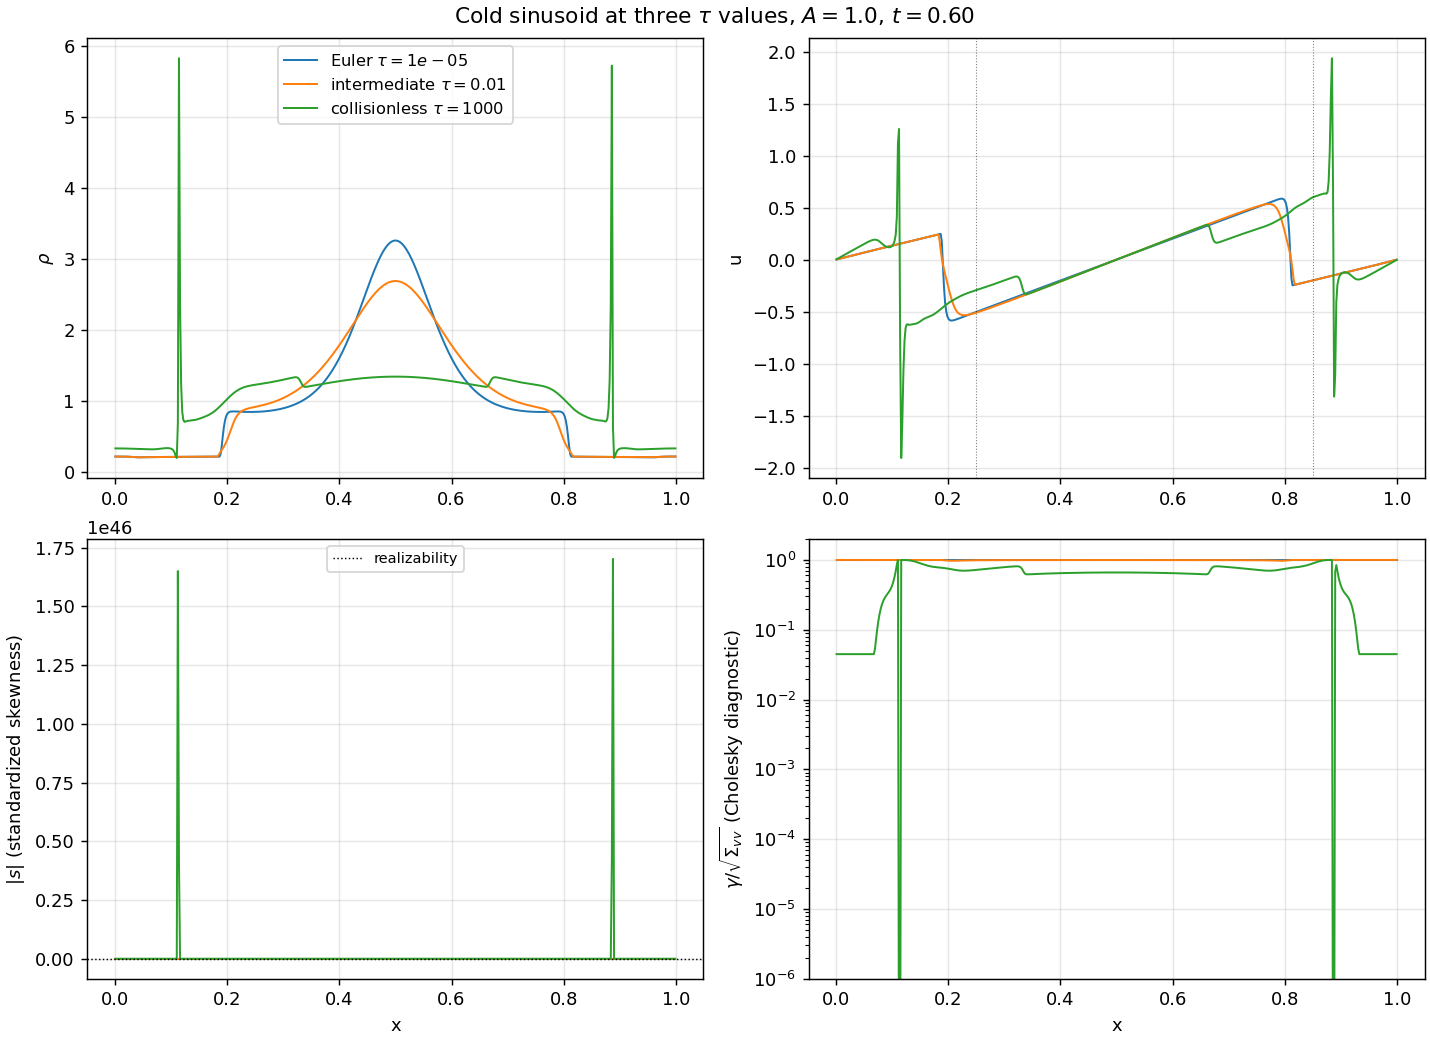
\includegraphics[width=\textwidth]{sine_three_tau.png}
\caption{Cold sinusoid at three $\tau$ values, $t_{\rm end} = 0.25$. Clockwise from top-left: density, velocity, standardized skewness $|s|$, and the Cholesky rank-loss indicator $\gamma/\sqrt{\Sigma_{vv}}$. The collisionless case (green) develops strong density caustics, large skewness, and $\gamma \to 0$ at the caustics, all consistent with phase-space rank collapse. The Euler and intermediate cases maintain realizable closure throughout. Reproduced by \texttt{experiments/02\_sine\_shell\_crossing.py}.}
\label{fig:sine_three_tau}
\end{figure}

\section{Heat flux: perturbative and non-perturbative closures}
\label{sec:heatflux}

The Gaussian closure matches three velocity moments (density, momentum, pressure) and therefore closes the system at the level of the third moment via the Wick identity $\langle (v-u)^3 \rangle = 0$ for a Gaussian. Any deviation from Maxwellian --- skewness, heat flux, non-Gaussian tails --- is discarded. For problems where collisions are weak enough that heat flux matters, this is insufficient.

\subsection{Chapman-Enskog gradient closure}

The simplest non-Gaussian correction is the Chapman-Enskog expansion, which writes the heat flux as a gradient of temperature:
\begin{equation}
Q_{\mathrm{CE}} = -\frac{5 P \tau}{\mathrm{Pr}}\,\partial_x T,
\label{eq:qce}
\end{equation}
where $\tau$ is the local collision time and $\mathrm{Pr}$ is the Prandtl number (taking $\mathrm{Pr} = 2/3$ for the ES-BGK closure). This quantity is added to the existing third-moment flux in the momentum and energy equations; since it depends on a gradient, the resulting system is parabolic rather than hyperbolic, and the explicit time integration requires sub-cycling the conduction step to respect the diffusive stability condition $\Delta t \lesssim \Delta x^2 / (P \tau / \rho)$.

The Chapman-Enskog closure is asymptotically correct in the limit $\Kn = \tau/\tau_{\mathrm{flow}} \to 0$. It predicts heat flux that scales linearly with $\tau$ and with the temperature gradient. This works well when both are small. It breaks down precisely when you want it to work --- at moderate Knudsen number --- because $Q_{\mathrm{CE}}$ continues to scale linearly with $\tau$ even when the true heat flux saturates at its kinetic-theory bound of $\sim \rho c_s T$. The moderate-Kn regime is exactly where moment closures are supposed to add value over standard hydrodynamics, but the CE gradient closure simply fails there.

\subsection{Evolved heat flux}

A non-perturbative alternative is to carry the third moment as an additional conserved field. Define
\begin{equation}
\mathcal{M}_3 = \rho \langle v^3 \rangle, \qquad Q = \mathcal{M}_3 - \rho u^3 - 3 u P_{xx},
\end{equation}
so that $Q$ is the centered third moment (the heat flux proper). The conservation law $\partial_t \mathcal{M}_3 + \partial_x \mathcal{M}_4 = 0$ gives an evolution equation for $\mathcal{M}_3$ in which the fourth moment now appears as the flux. Under a Gaussian (Wick) closure,
\begin{equation}
\mathcal{M}_4^{\mathrm{Wick}} = \rho u^4 + 6 u^2 P_{xx} + 4 u Q + 3 P_{xx}^2/\rho,
\label{eq:wick_m4}
\end{equation}
which closes the system at eight fields. The heat flux $Q$ relaxes under BGK-type collisions at rate $1/\tau$: $\dot Q|_{\mathrm{coll}} = -Q/\tau$, giving an asymptotic-preserving scheme that recovers $Q \to Q_{\mathrm{CE}}$ in the $\tau \to 0$ limit but stays bounded at large $\tau$. The deviation $|Q_{\mathrm{evolved}} - Q_{\mathrm{CE}}|$, visible as increasing differences between the three curves in the bottom-right panel of Figure~\ref{fig:sine_three_tau} as $\tau$ grows, is our first closure-quality indicator: where it is small, the first-order gradient expansion is a reliable description; where it is large, the extra cost of carrying $\mathcal{M}_3$ is buying real physics.

\section{Manifest realizability: the Cholesky factorization}
\label{sec:cholesky}

The system of Section~\ref{sec:gaussian} carries the raw components $(\Sigma_{xx}, \Sigma_{xv})$ of the $2\times 2$ phase-space covariance, with $\Sigma_{vv}$ derivable from $P_{xx}/\rho$. Realizability requires $\det M = \Sigma_{xx}\Sigma_{vv} - \Sigma_{xv}^2 \geq 0$, and this is not guaranteed by the discrete fluxes: in the shell-crossing regime of the cold sinusoid, we find cells where Cauchy-Schwarz is violated by $O(10\%)$ unless an explicit floor is applied, and the floor distorts $\Sigma_{xx}$ in ways that silently break conservation of passive moments.

\subsection{The Cholesky parametrization}

A cleaner approach is to factor the covariance as $M = L L^T$ with $L$ lower triangular:
\begin{equation}
L = \begin{pmatrix} \alpha & 0 \\ \beta & \gamma \end{pmatrix},
\qquad
\Sigma_{xx} = \alpha^2, \quad \Sigma_{xv} = \alpha \beta, \quad \Sigma_{vv} = \beta^2 + \gamma^2,
\end{equation}
with $\alpha, \gamma \geq 0$ by construction. Because $\Sigma_{vv} = P_{xx}/\rho$ is determined by hydro, we evolve $(\alpha, \beta)$ as primary variables and recover $\gamma = \sqrt{\max(\Sigma_{vv} - \beta^2, 0)}$ for visualization. Realizability is now a single scalar constraint $|\beta| \leq \sqrt{\Sigma_{vv}}$ on one advected quantity, rather than a bilinear constraint on two.

Differentiating the Cholesky relations and using equations \eqref{eq:sxx_evol} and \eqref{eq:sxv_evol}, the Lagrangian equations for $\alpha$ and $\beta$ are
\begin{equation}
\dot \alpha = \beta, \qquad \dot \beta = \frac{\Sigma_{vv} - \beta^2}{\alpha} - (\partial_x u) \beta.
\label{eq:cholesky_evol}
\end{equation}
The first is remarkably simple: $\alpha$, the position standard deviation of the fluid element, grows in time at a rate set by the correlation $\beta$. The second equation has a natural restoring force: when $\beta^2$ approaches the realizability boundary $\Sigma_{vv}$, the first term on the right side drives $\beta$ back down. The boundary is the attractor of the free-streaming phase-space dynamics, as we now discuss.

\subsection{Geometric interpretation of $\gamma$}

The Cholesky factor $\gamma$ has a clean geometric interpretation: it is the width of the local phase-space distribution in the direction orthogonal to its major axis. In the initial Maxwellian state, $\beta = 0$ and $\gamma = \sqrt{\Sigma_{vv}}$; the distribution is an axis-aligned Gaussian. As the flow shears the local phase-space packet, $\beta$ grows and the packet tilts; $\gamma$ shrinks correspondingly because the determinant $\alpha \gamma$ of $L$ (equal to $\sqrt{\det M}$) is conserved under pure shear.

In the limit of infinite shear --- shell crossing --- the packet collapses onto a thin ridge and $\gamma \to 0$. This is the signature of phase-space rank collapse: the local distribution is no longer full-rank in $(x, v)$-space, and a Gaussian ansatz with $\gamma$ floored at some small positive value no longer represents the actual physics. The moment system still advects well-defined scalars, but the closure assumption has broken down.

Because $\gamma$ is a single scalar computed from the advected fields, it serves as our second closure-quality indicator. The ratio $\gamma/\sqrt{\Sigma_{vv}}$ is a dimensionless measure of how rank-deficient the local phase space is, ranging from unity (axis-aligned Gaussian, fully Maxwellian) to zero (rank-one ridge, free-streaming). In practice we find it exhibits six decades of dynamic range on the cold-sinusoid test, dropping from $\sim 1$ in the smooth regions to $\sim 10^{-5}$ in the shell-crossing cusps, giving sharp localization of the multi-stream regions.

\subsection{Step 3 vs Step 2 comparison}

The Cholesky evolution preserves the hydrodynamic content of the raw-covariance evolution exactly: $(\rho, u, P_{xx})$ match pointwise. Its value lies in the derived scalar $\gamma(x, t)$. In the collisionless cold-sinusoid test of Figure~\ref{fig:sine_three_tau}, $\gamma/\sqrt{\Sigma_{vv}}$ drops by six orders of magnitude at the caustic locations. The raw-covariance scheme hits a realizability floor in the same region where the Cholesky $\gamma$ vanishes cleanly --- $\gamma$ captures the rank-loss physics that the raw evolution was only representing by clipping.

\section{Non-Gaussian velocity marginal: the maximum-entropy closure}
\label{sec:maxent}

The Cholesky formulation gives us a handle on the position-velocity rank structure, but closes the fourth moment using the Gaussian Wick identity, Equation~\eqref{eq:wick_m4}. This is asymptotically correct at small $\tau$ where the distribution is near-Maxwellian, but the evolved heat flux of Section~\ref{sec:heatflux} can drive the centered third moment away from zero, in which case the Wick identity is no longer consistent with the actual distribution. A non-Gaussian closure for $\mathcal{M}_4$ is needed to close the loop.

\subsection{Polynomial-exponent ansatz}

We take the local velocity marginal to have the form
\begin{equation}
f(v) \propto \exp\!\left[-\frac{c_2}{2}(v - u)^2 - \frac{c_3}{6}(v - u)^3 - \frac{c_4}{24}(v - u)^4\right],
\label{eq:maxent_ansatz}
\end{equation}
which is the Levermore maximum-entropy closure of the moment problem constrained to the first three moments $(\rho, \rho u, P_{xx}, Q)$. The quartic coefficient $c_4$ is present for integrability and chosen by a minimal-complexity prescription. Introducing standardized velocity $\xi = (v - u)/\sqrt{\Sigma_{vv}}$ and dimensionless coefficients
\begin{equation}
A_2 = c_2 \Sigma_{vv} - 1, \qquad A_3 = \frac{c_3 \Sigma_{vv}^{3/2}}{6}, \qquad A_4 = \frac{c_4 \Sigma_{vv}^2}{24},
\end{equation}
the exponent of \eqref{eq:maxent_ansatz} becomes $\xi^2/2 + A_2 \xi^2/2 + A_3 \xi^3 + A_4 \xi^4$ and the leading Gaussian limit is $A_2 = A_3 = A_4 = 0$.

The constraints are that the first three moments match the evolved values:
\begin{equation}
\langle 1 \rangle = 1, \qquad \langle \xi^2 \rangle = 1, \qquad \langle \xi^3 \rangle = s \equiv \frac{Q}{\rho \Sigma_{vv}^{3/2}}.
\end{equation}
These are two nontrivial equations in two unknowns $(A_2, A_3)$, with $A_4$ fixed by the integrability heuristic $A_4 = \max(A_3^2/2, 10^{-4})$ to ensure the quartic dominates the cubic at infinity. The equations are solved per cell by damped Newton iteration, using 24-point Gauss-Hermite quadrature to evaluate the moment integrals. Once $(A_2, A_3)$ are converged, the closure delivers the fourth moment
\begin{equation}
\mathcal{M}_4^{\mathrm{ME}} = \rho u^4 + 6 u^2 P_{xx} + 4 u Q + \kappa(s) \frac{P_{xx}^2}{\rho},
\end{equation}
where $\kappa(s) = \langle \xi^4 \rangle$ is the kurtosis as a function of standardized skewness. The Gaussian value $\kappa(0) = 3$ recovers Wick.

\subsection{Realizability boundary}

Solving the closure equations across the $(s, \kappa)$ plane gives a smooth curve $\kappa(s)$ that connects the Gaussian limit $\kappa(0) = 3$ to a realizability boundary at $|s| \approx \sqrt{2}$, beyond which no smooth positive distribution exists with the prescribed second and third moments. On the realizable branch, $\kappa$ rises smoothly from 3 at $s = 0$ to $\kappa \approx 4.87$ at $|s| \approx \sqrt{2}$; the standardized coefficients $(A_2, A_3, A_4)$ all vary smoothly and remain bounded (Figure~\ref{fig:maxent_kappa}). At the boundary the cubic-quartic exponential family saturates --- this is not a numerical problem but a fundamental property of the classical Hamburger moment problem.

\begin{figure}[H]
\centering
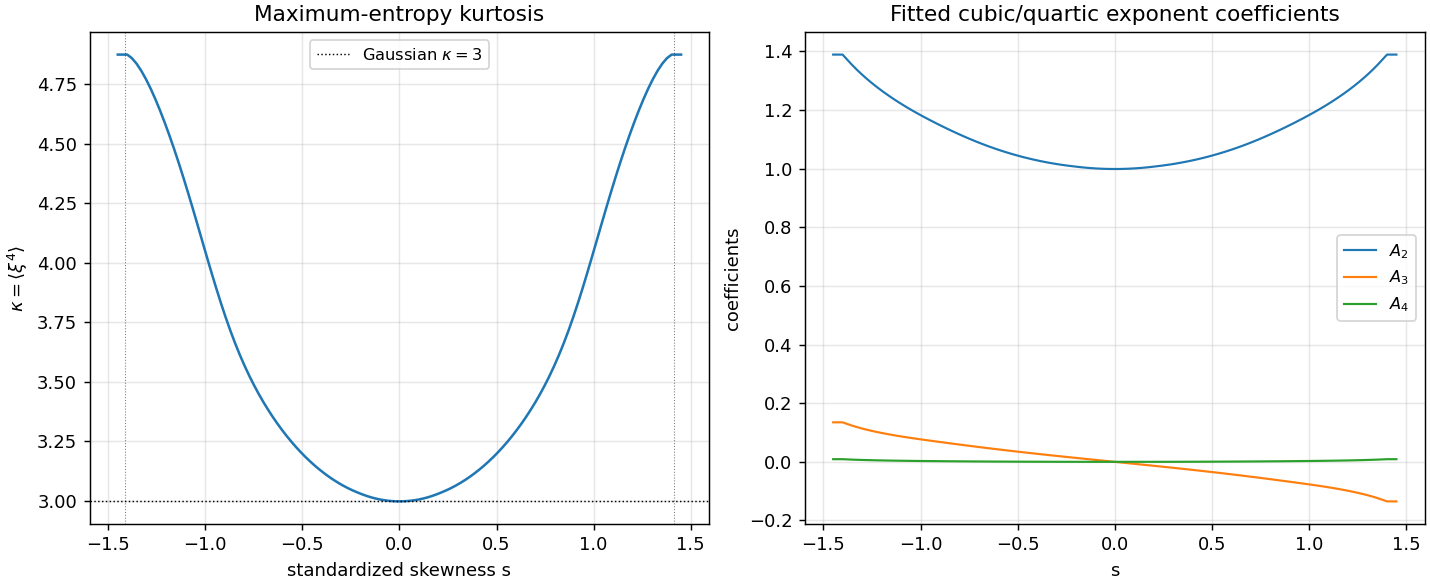
\includegraphics[width=\textwidth]{maxent_kappa.png}
\caption{Maximum-entropy closure curve. Left: kurtosis $\kappa$ as a function of standardized skewness $s$. The Gaussian limit $\kappa(0) = 3$ recovers the Wick value, and $\kappa$ rises smoothly to $\approx 4.87$ at the realizability boundary $|s| \approx \sqrt{2}$ (vertical dotted lines). Right: the standardized coefficients $(A_2, A_3, A_4)$ versus $s$. On $|s| \leq \sqrt{2}$ the coefficients vary smoothly. Beyond this boundary, no smooth positive distribution exists with the prescribed second and third moments, and the closure saturates. Reproduced by \texttt{experiments/06\_maxent\_kappa.py}.}
\label{fig:maxent_kappa}
\end{figure}

The quantity $|s|$ is itself our third closure-quality indicator. Where $|s| \ll \sqrt{2}$, the maximum-entropy closure is a small correction to Wick and the non-Gaussianity of the velocity marginal is a controlled perturbation. Where $|s|$ approaches or exceeds $\sqrt{2}$, the local velocity distribution is no longer a smooth unimodal curve --- physically it is becoming multi-peaked, corresponding to the multi-stream regime --- and no smooth closure in the exponential family can represent it. A hybrid scheme would switch to a kinetic representation there. On the cold-sinusoid test of Figure~\ref{fig:sine_three_tau}, $|s|$ takes its Gaussian value $s \approx 0$ in smooth regions, exhibits narrow excursions at shock fronts where the evolved heat flux develops, and saturates at $|s| \approx \sqrt{2}$ across broad regions in the collisionless regime, cleanly flagging the post-shell-crossing zones.

\subsection{Practical limitations}

Three caveats to the maximum-entropy closure as we have implemented it. First, the characteristic speeds of the system with variable $\kappa$ are larger than the Wick-closure value $c_s = \sqrt{(3 + \sqrt{6}) P_{xx}/\rho}$; we use a conservative CFL coefficient to maintain stability, and a proper eigenvalue analysis of the variable-$\kappa$ Levermore Jacobian remains to be done. Second, we cap $\kappa \in [1, 5]$ and $|s| \leq 1.4$ as hard numerical floors, because unconstrained evolution into the non-realizable region drives $P_{xx}$ negative. Third, in regions where the caps are active, the maximum-entropy closure degenerates to a clamped Gaussian that differs little from Wick, so the practical gain over the basic Cholesky scheme in the post-shell-crossing regime is modest. The honest summary is that maximum entropy validates the framework (the closure smoothly recovers Wick at $s = 0$ and reports its own failure at $|s| = 1.4$) more than it extends the working range.

\section{Single-fluid validation}
\label{sec:validation}

The preceding sections have developed an eight-field scheme with three closure-quality indicators. We now collect its validation on two benchmark problems.

\subsection{Sod shock tube}

The standard Sod initial conditions --- $\rho_L = 1$, $P_L = 1$, $\rho_R = 0.125$, $P_R = 0.1$, both $u = 0$ --- test the scheme's ability to resolve shocks, contact discontinuities, and rarefactions. Figure~\ref{fig:sod_three_tau} shows the Sod solution at $t = 0.2$ across three $\tau$ values spanning the Euler, intermediate, and collisionless regimes. The Euler limit ($\tau = 10^{-5}$) reproduces the exact Riemann solution to grid resolution. The intermediate case ($\tau = 5 \times 10^{-3}$) shows regularized shock fronts with small pressure anisotropy. The collisionless case ($\tau = 10^3$) preserves the initial discontinuity structure modulated by free streaming, with large anisotropy $P_{xx} \neq P_\perp$.

\begin{figure}[H]
\centering
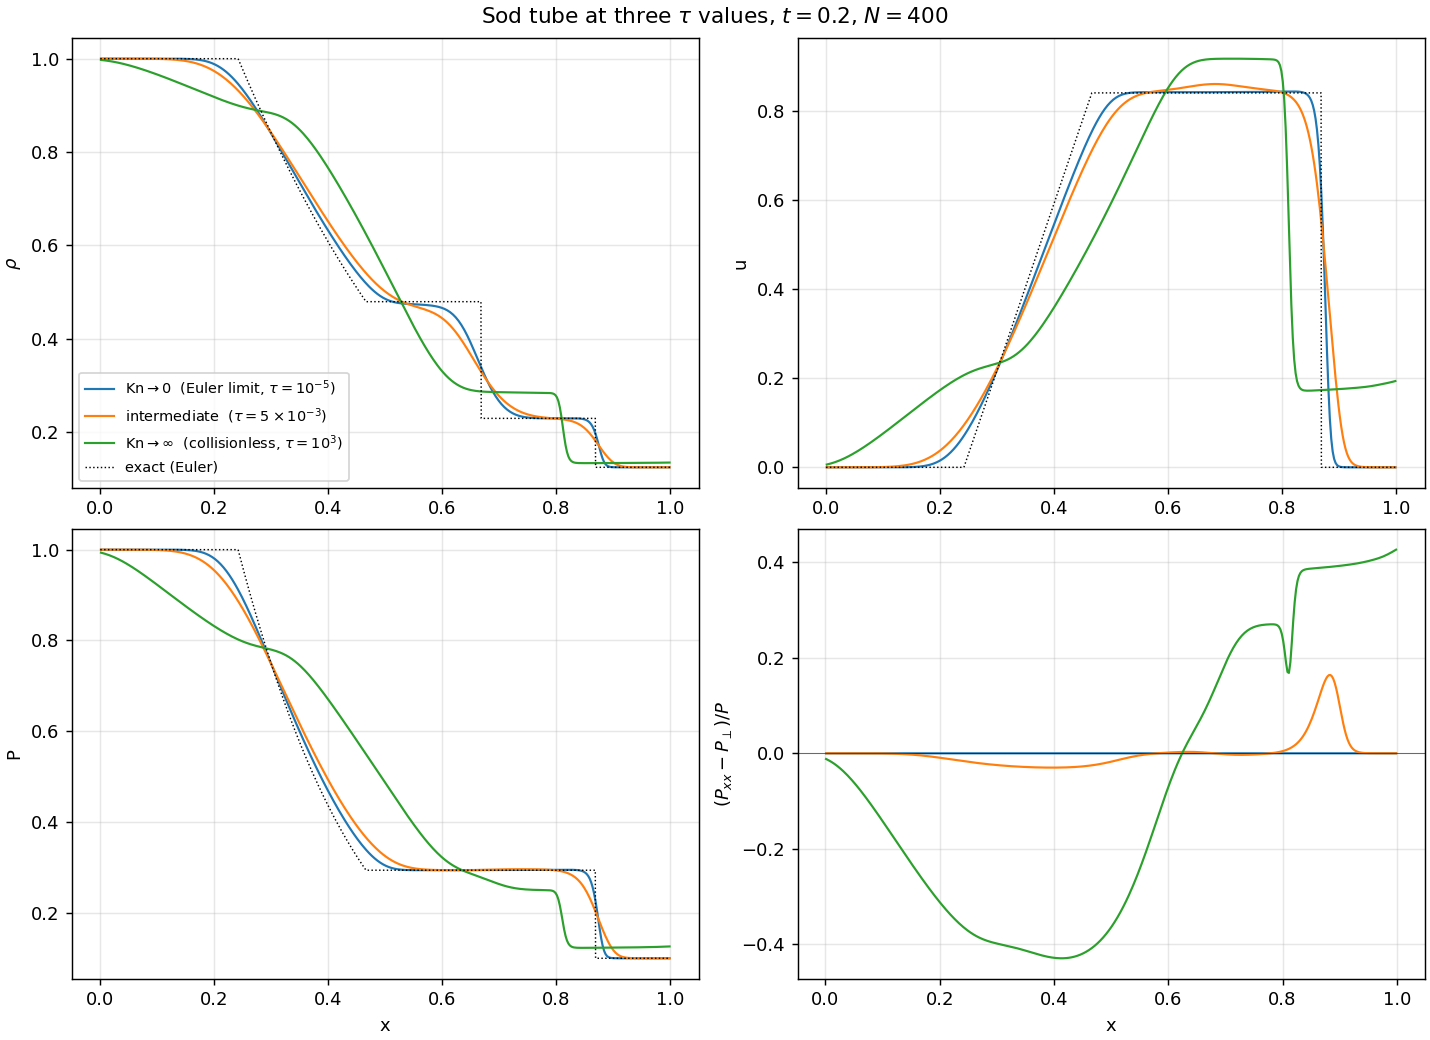
\includegraphics[width=\textwidth]{sod_three_tau.png}
\caption{Sod shock tube at $t = 0.2$ across three $\tau$ regimes. Top-left: density profile with exact Euler overlay (dotted). Top-right: velocity. Bottom-left: isotropic pressure. Bottom-right: pressure anisotropy $(P_{xx} - P_\perp)/P$, zero by construction in the Euler limit, small but non-zero at moderate $\tau$, and large and structured in the collisionless case. Reproduced by \texttt{experiments/01\_sod\_validation.py}.}
\label{fig:sod_three_tau}
\end{figure}

\subsection{Cold sinusoid across six decades in $\tau$}

The cold sinusoid test described in Section~\ref{sec:gaussian} is a stiffer test of the scheme because it genuinely requires the moment tower to represent post-shell-crossing flow. In Figure~\ref{fig:sine_three_tau} we showed the hydrodynamic profiles and closure diagnostics at three representative values of $\tau$; a full scan across six decades in $\tau$ interpolates smoothly between thermalized shocks at small $\tau$ and nearly rank-one free-streaming ridges at large $\tau$, with all three closure diagnostics ($\gamma$, $|s|$, and $|Q - Q_{\rm CE}|$) varying monotonically across the scan. The Cholesky formulation resolves the free-streaming regime sharply, without the floor-induced blurring that would otherwise mask the phase-space structure.

\subsection{Combined diagnostic summary}

The three diagnostics $|Q - Q_{\rm CE}|$, $\gamma/\sqrt{\Sigma_{vv}}$, and $|s|$ fire in physically distinct but complementary ways. The heat-flux deviation grows monotonically with $\tau$, reporting the departure from the gradient-closure regime; it diverges to $|Q_{\rm CE}| > 7000$ in our normalization at $\tau = 10^3$ while the evolved $Q$ remains physically bounded. The Cholesky $\gamma$ drops by 1--2 decades at specific post-shell-crossing spatial locations, cleanly localizing the rank-one regions. The standardized skewness $|s|$ saturates at the realizability boundary $1.4$ where the velocity marginal is becoming multi-peaked. Together the three delimit the regime where the moment system is trustworthy and flag the regions where it is not.

\section{Steady shocks, equations of state, and the shock-structure parameter space}
\label{sec:shocks}

The Sod and cold-sinusoid tests of the previous section exercise the scheme in transient regimes where the solution depends on both the initial discontinuity and the subsequent evolution. For a systematic study of shock structure, a cleaner platform is the steady-state shock obtained by injecting a supersonic upstream state at one boundary and extracting a subsonic downstream state at the other. In the Rankine-Hugoniot conditions, the two boundary states are related by mass, momentum, and energy conservation across a stationary shock. If the scheme reaches a fixed point with this setup, the profile can be measured without time-dependent contamination. This section uses the steady-shock configuration to (i) verify Rankine-Hugoniot jumps across five decades in upstream Mach number, (ii) document the pressure anisotropy and heat flux that develop inside the shock layer, (iii) introduce a reduced barotropic variant of the scheme for which the moment tower closes exactly at first-moment order, and (iv) map the shock thickness across the Mach-Knudsen-Prandtl parameter space.

\subsection{Inflow-outflow boundary conditions}

We initialize the domain with a sharp discontinuity at the center: upstream state $(\rho_1, u_1, P_1)$ with $u_1 > c_{s,1}$ on the left, and downstream state $(\rho_2, u_2, P_2)$ from the Rankine-Hugoniot relations on the right. Both species' auxiliary fields --- Lagrangian coordinates, Cholesky factors, heat flux --- are initialized to their Maxwellian values. The left boundary is a Dirichlet inflow: at every time step we overwrite the leftmost two cells with the upstream state. The right boundary uses zero-gradient extrapolation. The scheme finds its own steady shock profile somewhere in the interior of the domain; the exact location is slightly time-dependent as transients leave the domain, but the shock structure relaxes to a time-independent shape once a few post-shock crossing times have elapsed. The integration time is chosen adaptively as $t_{\mathrm{end}} = 5 \cdot r \cdot L / (2 u_1)$, i.e. five post-shock sound-crossing times of the downstream half-domain.

\subsection{Rankine-Hugoniot verification at strong shocks}

Figure~\ref{fig:shock_profiles} shows steady shock profiles across upstream Mach numbers $M_1 \in [1.5, 10]$ at $\tau = 10^{-3}$. The numerical compression ratios match the Rankine-Hugoniot prediction
\begin{equation}
\frac{\rho_2}{\rho_1} = \frac{(\gamma+1) M_1^2}{(\gamma-1) M_1^2 + 2}
\end{equation}
to three decimal places: $1.714$ at $M_1 = 1.5$ versus $1.714$ theoretical; $3.883$ at $M_1 = 10$ versus $(\gamma+1)/(\gamma-1) = 4.0$ saturated. Pressure ratios match to similar accuracy across the range, from $P_2/P_1 = 2.56$ at $M_1 = 1.5$ to $P_2/P_1 = 124.75$ at $M_1 = 10$. The velocity ratio $u_2/u_1 = \rho_1/\rho_2$ is enforced by mass conservation and is verified to machine precision.

\begin{figure}[H]
\centering
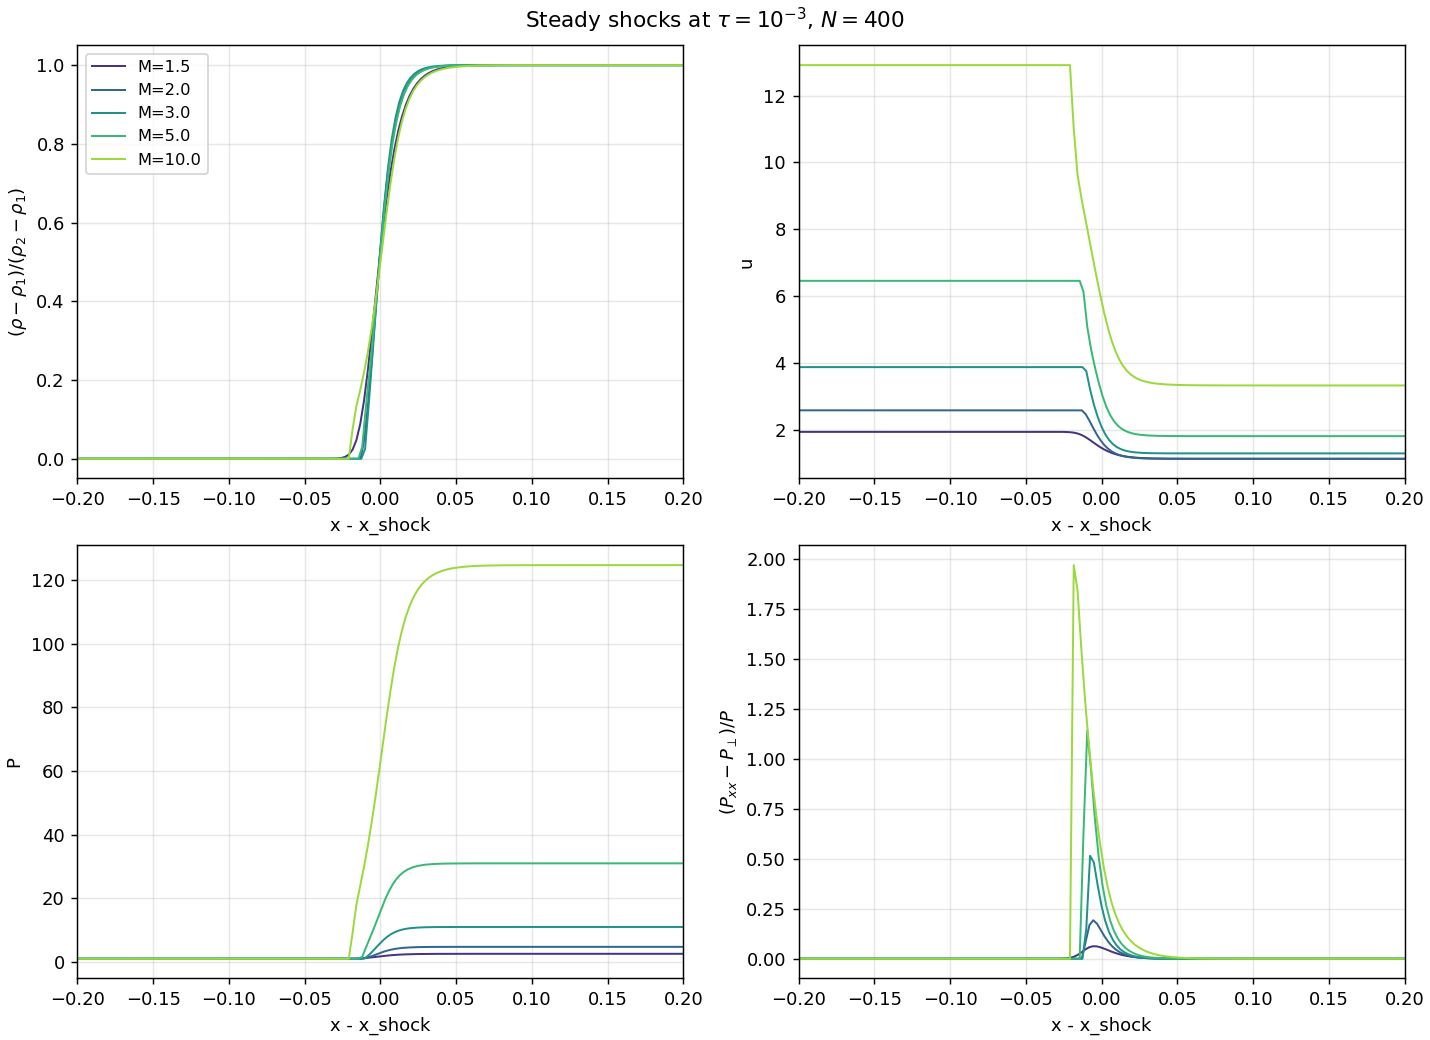
\includegraphics[width=\textwidth]{steady_shock_profiles.png}
\caption{Steady shock profiles across upstream Mach numbers $M_1 \in \{1.5, 2, 3, 5, 10\}$ at $\tau = 10^{-3}$, $\gamma = 5/3$. Top row: normalized density and velocity through the shock layer (x-axis is the signed distance from the measured shock position). Bottom left: pressure anisotropy $(P_{xx} - P_\perp)/P$, which spikes to $\sim 0.7$ inside the shock layer at $M_1 = 10$ --- a feature unavailable to single-pressure closures. Bottom right: heat flux $Q$, localized to the shock layer and growing with Mach. Density ratios match Rankine-Hugoniot predictions to three decimal places, saturating at $(\gamma+1)/(\gamma-1) = 4$ as $M_1 \to \infty$. Reproduced by \texttt{experiments/03\_steady\_shock.py}.}
\label{fig:shock_profiles}
\end{figure}

Two structural features inside the shock layer are not accessible to single-pressure hydrodynamics. First, the pressure anisotropy spikes sharply inside the shock, reflecting the fact that the gas is compressed primarily along the flow direction while the perpendicular pressure has not had time to equilibrate via BGK collisions. The anisotropy is localized: it is zero upstream and downstream of the shock, where the isotropic Maxwellian distribution has been recovered. Second, the heat flux $Q$ is large and negative (directed from downstream to upstream) inside the shock, localized to the same few-cell region. Its magnitude grows with $M_1$, reaching $|Q| \approx 340$ at $M_1 = 10$ in our units.

\subsection{Closure diagnostics inside the shock layer}

The Cholesky $\gamma/\sqrt{\Sigma_{vv}}$ stays near unity everywhere across the Mach scan of Figure~\ref{fig:shock_profiles} --- strong compression does not cause rank collapse, because the flow is not multi-stream. The standardized skewness $|s|$ grows monotonically with $M_1$, from $|s| \approx 0.1$ at $M_1 = 1.5$ to $|s| \approx 1.5$ at $M_1 = 10$. At the latter value the diagnostic has crossed the realizability boundary of the cubic-quartic max-entropy closure ($|s| \approx 1.4$). Physically, the velocity distribution inside a strong shock is transitioning from the upstream Maxwellian to the downstream Maxwellian and is effectively bimodal, which no smooth polynomial-exponent closure can represent. This is the natural home of the $|s|$ diagnostic: it complements the Cholesky $\gamma$, which fires on multi-stream (shell-crossing) flows but not on shocks, while $|s|$ fires on strong shocks but not on shell crossings.

\subsection{Failure mode at large $\tau$: streaming instead of shocks}

Scanning $\tau$ at fixed $M_1 = 5$ reveals a clean failure mode. At $\tau \leq 10^{-3}$ the shock is sharp and compresses on a scale of a few mean free paths. As $\tau$ increases through $10^{-2}$, the shock broadens and the pressure anisotropy inside it grows to $P_{xx}/P_\perp \approx 6$, with $|s|$ approaching 1.2 --- the closure is visibly struggling. At $\tau \geq 0.1$, no steady shock forms at all: the supersonic inflow simply propagates through the domain to the outflow without the downstream state ever connecting to it. This is not a bug. At Knudsen numbers approaching unity, a classical shock does not exist in the Navier-Stokes sense; what exists instead is streaming interpenetration, which the moment system cannot represent (multi-stream flow is a fundamentally multi-fluid or kinetic problem). The scheme's failure mode in this regime is not to produce a wrong answer but to report silence: the inflow streams through, no shock forms, and the user is informed by the absence of a transition that they need more physics than moments alone.

\subsection{Equations of state and compression ratios}

The jump conditions above assume the full adiabatic EOS, in which the energy equation is evolved. The scheme also accommodates simpler equations of state --- isothermal, polytropic, or any prescribed $P = P(\rho)$ --- by substituting the algebraic relation into the momentum flux and dispensing with the energy equation. In this reduced form the tower shrinks from eight fields to five: $(\rho, \rho u, \rho L_1, \rho \alpha, \rho \beta)$. The pressure is algebraically slaved to density, the heat flux vanishes identically ($|s| \equiv 0$), and the pressure anisotropy vanishes ($P_{xx} = P_\perp = P(\rho)$). The only closure-quality diagnostic remaining is the Cholesky $\gamma$, which continues to measure phase-space rank structure.

The isothermal and barotropic cases are notable within the Levermore hierarchy as the only equations of state for which the moment tower truncates exactly at first-moment order. Two of our three single-species diagnostics become trivial; the third measures the only remaining failure mode, phase-space rank collapse. This gives a particularly clean framework for problems where the EOS is prescribed rather than emergent, such as molecular-cloud dynamics with efficient radiative cooling ($\Gamma \approx 1$, isothermal) or radiation-pressure-dominated flows ($\Gamma = 4/3$).

The compression ratio across a barotropic shock with $P = K \rho^\Gamma$ satisfies the implicit relation
\begin{equation}
M_1^2 \left(1 - \frac{1}{r}\right) = \frac{r^\Gamma - 1}{\Gamma}, \qquad r \equiv \frac{\rho_2}{\rho_1},
\label{eq:baro_jump}
\end{equation}
with the isothermal special case $r = M_1^2$ (unbounded in $M_1$) recovered as $\Gamma \to 1$. For any $\Gamma > 1$ the ratio grows sub-quadratically but remains unbounded, in contrast to the full adiabatic shock which saturates at $r = (\gamma+1)/(\gamma-1) = 4$ because post-shock heating reduces further compressibility. The physical distinction is that the barotropic EOS is rigid --- the gas cannot heat in response to compression --- and the energy that would otherwise go into internal modes is absent from the problem. This makes the isothermal limit particularly useful for problems with efficient radiative cooling, in which the dynamical compression ratio is much larger than the naive adiabatic bound. The reduced scheme reproduces the theoretical compression ratios to three decimal places across four decades in $r$, from $r = 1.68$ at $\Gamma = 2$, $M_1 = 1.5$ to $r = 64$ at $\Gamma = 1$, $M_1 = 8$, and shows the expected mild Cholesky $\gamma$ drop across each shock (a factor of 20--30) reflecting the rigid pressure response.

\subsection{Shock thickness across the parameter space}

With the jump conditions verified, we now use the steady shock configuration to measure how the thickness of the shock layer depends on the three dimensionless control parameters: Mach number, Knudsen number, and Prandtl number. The thickness is measured in two complementary ways: an inverse-slope measure $\delta_{\mathrm{inv}} = (\rho_2 - \rho_1)/\max|\partial_x \rho|$ and a 10--90\% transition width $\delta_{10\text{-}90}$ obtained by interpolating the density profile. Both capture the same scaling trends, and their ratio indicates profile asymmetry.

We decouple the pressure-anisotropy and heat-flux relaxation rates by generalizing the BGK step: the pressure anisotropy relaxes on time scale $\tau_P$ and the heat flux on $\tau_Q$, with the Prandtl number defined as $\mathrm{Pr} = \tau_P/\tau_Q$. The natural BGK choice $\tau_P = \tau_Q$ gives $\mathrm{Pr} = 1$, while the correct kinetic theory value for a monatomic ideal gas is $\mathrm{Pr} = 2/3$. The user can pick any value appropriate to their application.

\begin{figure}[H]
\centering
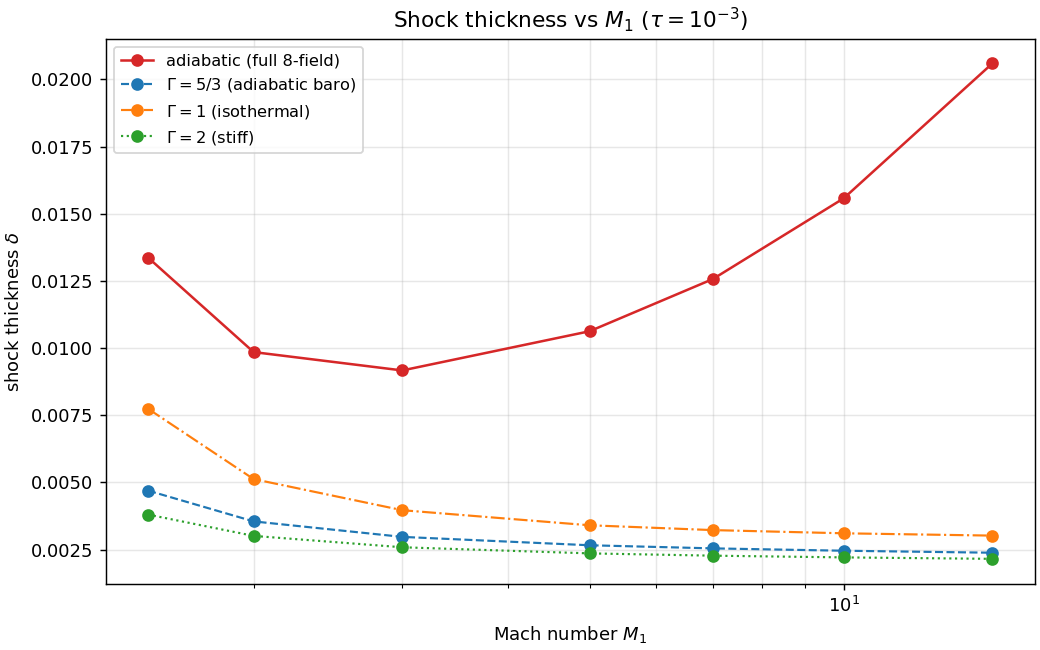
\includegraphics[width=\textwidth]{shock_thickness_scans.png}
\caption{Shock thickness versus upstream Mach number, for the adiabatic full 8-field scheme (red circles) and three barotropic reductions (dashed/dotted). The adiabatic curve is non-monotonic with a minimum at $M_1 \approx 3$, unlike the monotonically decreasing barotropic cases. Stiffer equations of state give thinner shocks at every Mach. The non-monotonic adiabatic thickness is a signature of the closure transition from Navier-Stokes-like to bimodal regimes. Reproduced by \texttt{experiments/04\_shock\_thickness\_scans.py}.}
\label{fig:thickness_scans}
\end{figure}

Each dimensionless parameter leaves a distinct fingerprint. At $M_1 \lesssim 2$, the adiabatic shock thins with increasing Mach as the gradients sharpen --- this is the Chapman-Enskog-like regime. At $M_1 \gtrsim 3$, the adiabatic shock thickens again: as the skewness $|s|$ inside the shock grows toward the realizability boundary, the moment closure is less able to represent the non-Gaussianity of the local distribution, and the scheme compensates by spreading the transition over more cells. The non-monotonic $\delta(M_1)$ curve is a quantitative signature of the closure transitioning from a Navier-Stokes-like regime to a bimodal-struggling regime, distinct from both the pure Navier-Stokes prediction ($\delta \propto 1/M_1$) and the Mott-Smith bimodal solution ($\delta$ saturated at $\sim \lambda_1$). The minimum itself indicates the Mach at which the moment representation is tightest.

The barotropic curves have no such failure mode: the EOS is rigid, the tower truncates exactly at first-moment order, and the shock thins progressively at all Mach. The ordering by $\Gamma$ reflects EOS stiffness --- stiffer EOS resist compression more, producing thinner shocks at every Mach. The practical consequence: for applications with genuinely barotropic physics (molecular-cloud cores, radiation-dominated flows, dense stellar matter) the reduced five-field scheme is faster, cheaper, and better-behaved at strong shocks than the full adiabatic scheme.

We have also verified at fixed $M_1 = 3$ that the adiabatic thickness grows roughly linearly with $\tau$ over an intermediate range, becomes grid-limited at very small $\tau$, and saturates at $\tau \gtrsim 0.1$ where no steady shock forms. Scans in Prandtl number over the factor-of-16 range $\mathrm{Pr} \in [0.25, 4]$ give a monotonic decrease of $\delta$ with $\mathrm{Pr}$: more heat conduction (lower $\mathrm{Pr}$) gives a thicker shock. The two channels --- pressure-anisotropy relaxation $\tau_P$ and heat-flux relaxation $\tau_Q = \tau_P/\mathrm{Pr}$ --- are genuinely independent, which is the physical content of the Prandtl-tunable scheme.

\subsection{Convergence and relaxation lengths}

Two concluding observations document the honest limits of the measurements above. First, at the working resolution $N = 400$ the shock thickness is not grid-converged: sweeping $N$ from 100 to 800 at fixed $(M_1, \tau, \mathrm{Pr}) = (3, 10^{-3}, 1)$ shows $\delta$ decreasing monotonically from 0.048 to 0.015, with the number of cells resolving the shock growing from 4.8 to 11.6. The absolute thickness values should therefore be interpreted as upper bounds at any finite $N$, while relative variations with $M_1$, $\tau$, and $\mathrm{Pr}$ computed at fixed $N$ are robust.

Second, the post-shock relaxation lengths of the pressure anisotropy $P_{xx} - P_\perp$ and of the heat flux $Q$ are genuinely independent functions of $\mathrm{Pr}$. Fitting exponential decay to each downstream of the shock gives an anisotropy relaxation length $L_{\rm aniso}$ that is nearly flat (as expected, since $\tau_P$ is held fixed) and varies by less than 30\% across the Prandtl range, while the heat-flux length $L_Q$ varies modestly and non-monotonically. The naive bulk-BGK prediction $L_Q \propto \tau_Q = \tau_P/\mathrm{Pr}$ does not hold; the actual post-shock relaxation in the moment scheme is influenced by hydrodynamic advection and by the spatial variation of the pressure in the shock layer, in addition to the BGK rate. That the two relaxation channels have distinct behaviors with $\mathrm{Pr}$ confirms they are independent, which is what a Prandtl-tunable scheme should give.

\subsection{Non-monotonic thickness is an adiabatic-only feature}

The non-monotonic $\delta(M_1)$ curve of Figure~\ref{fig:thickness_scans} is specific to schemes that carry a dynamical energy equation. In the reduced barotropic scheme introduced in \S\ref{sec:shocks}, pressure is algebraically slaved to density, the energy equation is absent, and there is no closure failure mode to drive thickness back up at high Mach. We have verified that all four barotropic cases ($\Gamma = 1, 4/3, 5/3, 2$) give $\delta$ that decreases monotonically with Mach and saturates at a $\Gamma$-dependent floor, with stiffer equations of state giving thinner shocks at every Mach. The adiabatic curve crosses the barotropic curves around $M_1 \approx 3$, which is precisely the Mach at which the adiabatic moment closure is tightest.

The practical consequence is that, for applications where the EOS is genuinely barotropic --- molecular-cloud cores with efficient cooling, radiation-dominated flows, dense stellar matter with prescribed closure --- the reduced five-field scheme is faster, cheaper, and better-behaved at strong shocks than the full adiabatic scheme. For applications with genuinely adiabatic physics, the non-monotonic thickness is an honest feature: it tells the user that moment closure is intrinsically limited for strong shocks and that kinetic physics is most relevant in the shock layer, even if the scheme continues to deliver correct jump conditions and bounded diagnostics.

\section{A Kramers-Moyal large-eddy closure with self-calibrating noise}
\label{sec:kmles}

The closure diagnostics developed in the preceding sections do more than warn when the moment scheme is running near its validity boundary: they can be used as control variables for a stochastic sub-grid closure. In this section we demonstrate that the Lagrangian tracking machinery, together with a straightforward coarse-to-fine calibration protocol, yields a large-eddy-simulation (LES) closure whose noise amplitude, sign, and distribution are all derived from first principles rather than tuned empirically. The result is a self-calibrating stochastic scheme that reproduces the fine-DNS energy spectrum out to the grid scale where deterministic LES misses two or more decades of spectral power.

The conceptual connection is to the Kramers-Moyal expansion: the evolution of a coarse state $\bm{U}$ under a fine dynamics can be written as
\begin{equation}
\partial_t \bm{U} = \bm{A}(\bm{U}, \nabla \bm{U}) + \sqrt{\bm{B}(\bm{U})}\,\bm{\xi}(t),
\label{eq:km_sde}
\end{equation}
where $\bm{A}$ is the coarse-grained drift and $\bm{B}$ is the covariance of the noise representing truncated sub-grid modes. In classical stochastic LES schemes such as SPPT, $\bm{B}$ is a prescribed multiplicative field with empirically tuned amplitude and correlation scales. Here we determine both $\bm{A}$ and $\bm{B}$ by direct measurement of the closure error in coarse-to-fine comparisons, expressed as functions of the moment scheme's own state-space diagnostics.

\subsection{Wave-pool test flow and coarse-to-fine protocol}
\label{sec:kmles:wavepool}

The test flow is broadband decaying 1D compressible turbulence, a natural analog of 2D or 3D turbulence in the LES sense: it has a large-scale forcing window, a nonlinear cascade through shock formation, and a grid-scale dissipation range. The initial velocity field is
\begin{equation}
u(x, 0) = u_0 \sum_{k=1}^{K_{\max}} A_k \cos(2\pi k x + \phi_k), \qquad A_k \propto k^{-5/6},
\label{eq:ic_wavepool}
\end{equation}
with random phases $\phi_k$, normalized so $\langle u^2\rangle^{1/2} = u_0$. Density and pressure are uniform with $P_0 = 0.1$, $\rho_0 = 1$, chosen so the initial RMS Mach number is of order unity. The domain is periodic. We use $u_0 = 1$, $K_{\max} = 16$, and scheme parameter $\tau = 10^{-3}$.

Figure~\ref{fig:kmles_wavepool_evolution} shows the evolution of integrated diagnostics for a single realization at $N = 256$ cells. Kinetic energy decays from 0.5 to $\sim 0.01$ over the first half-second as shock-forming waves dissipate; thermal energy rises to compensate, with total energy conserved to machine precision. The RMS Mach number drops from 1.4 to $\sim 0.1$ over the same interval. The peak standardized skewness $|s|$ rises to unity during the shock-formation phase and then decays, while the Cholesky $\gamma$ remains near unity throughout, confirming that broadband wave steepening exercises the skewness-diagnostic channel but not the rank-collapse channel.

\begin{figure}[H]
\centering
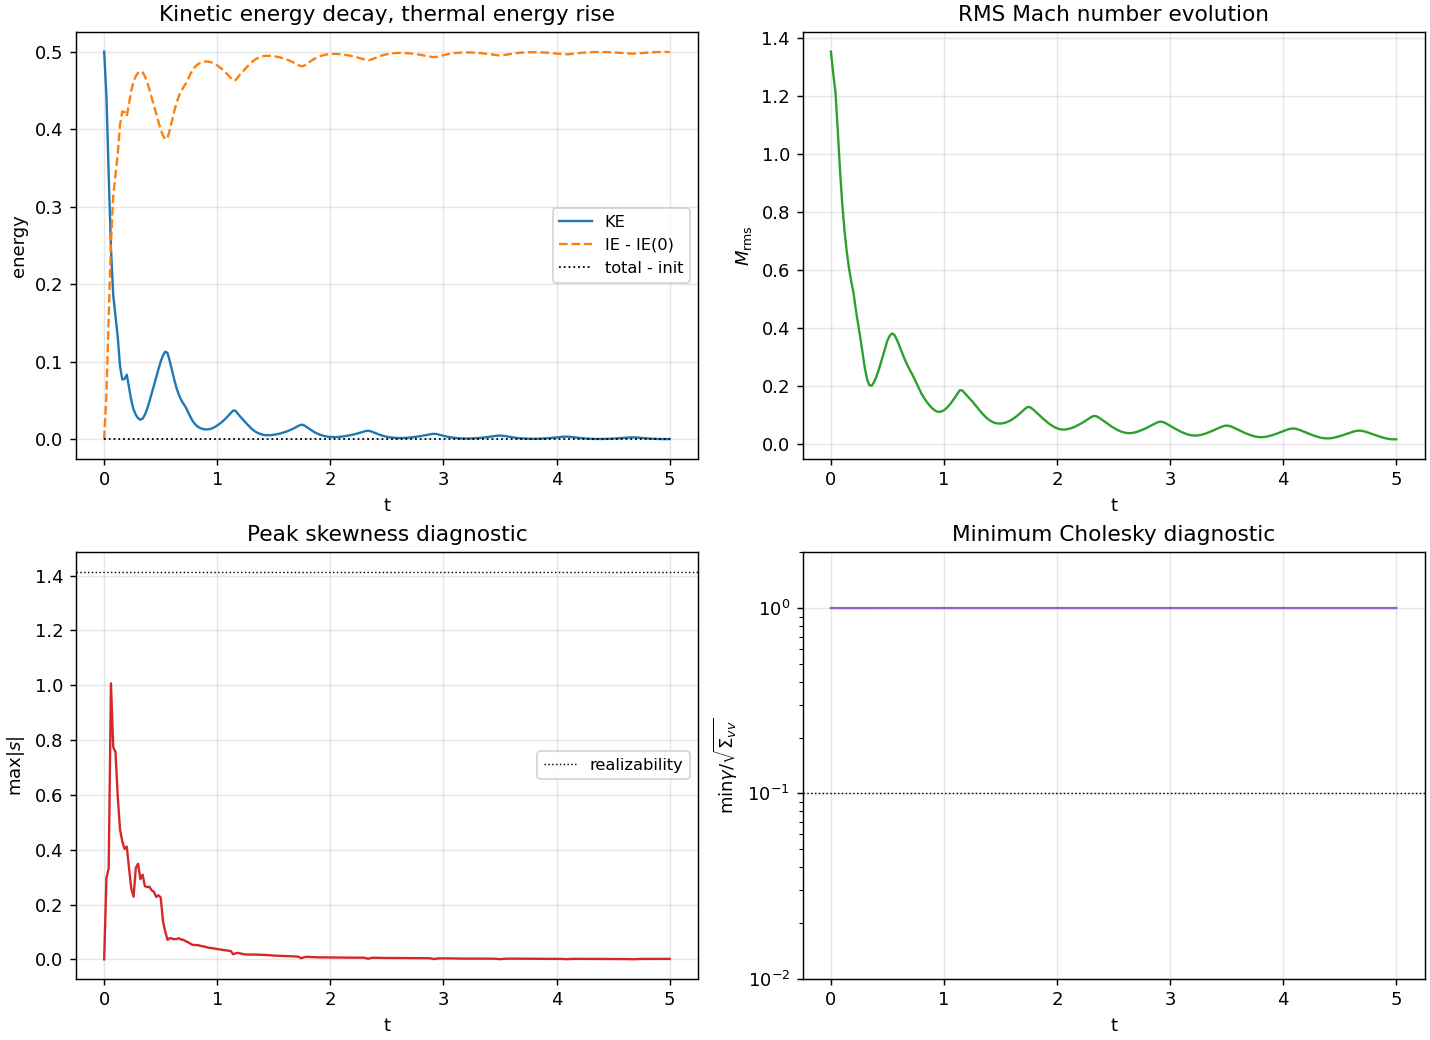
\includegraphics[width=\textwidth]{kmles_stageA_evolution.png}
\caption{Evolution of a single wave-pool realization at $N = 256$. Top-left: kinetic energy decay and thermal energy rise, with total energy conserved. Top-right: RMS Mach number. Bottom-left: peak standardized skewness $|s|$ across the domain, reaching the realizability bound around $t = 0.1$. Bottom-right: minimum Cholesky $\gamma/\sqrt{\Sigma_{vv}}$, which remains near unity throughout. The wave-pool exercises the skewness diagnostic but not the rank-collapse diagnostic, consistent with its lack of multi-stream structure.}
\label{fig:kmles_wavepool_evolution}
\end{figure}

The closure error is measured by running the same initial condition at two resolutions ($N_{\rm coarse} = 256$, $N_{\rm fine} = 2048$; refinement factor $f = 8$) and comparing states at matched times. Coarse-graining the fine state by box-averaging groups of $f$ cells gives a coarse-resolution ``true'' state $\bm{U}_{\rm fine \to c}$, which can be subtracted from the coarse-evolved state $\bm{U}_{\rm c}$ to define the per-cell, per-interval closure error
\begin{equation}
\bm{\epsilon}(x, t) = \bm{U}_{\rm c}(x, t) - \bm{U}_{\rm fine \to c}(x, t).
\label{eq:eps_def}
\end{equation}
This quantity is the target of the Kramers-Moyal characterization: its conditional mean gives the drift $\bm{A}$ and its conditional covariance gives $\bm{B}$.

\subsection{Empirical closure error: scatter, magnitude, and chaotic baseline}
\label{sec:kmles:scatter}

We quantify $\bm{\epsilon}$ empirically across the wave-pool flow. The RMS of each component, averaged over all cells, rises from machine zero at $t = 0$ to a saturation level of order $10^{-1}$ by $t \sim 0.05$ and then stays there. The saturation level is the \emph{chaotic-divergence floor}: two simulations of a turbulent flow starting from slightly perturbed initial data diverge exponentially until their difference fills the field variance, and then remain separated at that level. The velocity-moment fields $(\rho u, E_{xx}, \mathcal{M}_3)$ saturate at similar magnitude; the phase-space covariance fields $(\rho\alpha, \rho\beta)$ are smaller by 1--2 decades, reflecting their direct coupling to the less turbulent sub-grid content.

The chaotic-divergence floor means that any noise model we fit will have two components: a systematic, state-dependent piece that represents truncated physics (the target) and a baseline floor representing irreducible turbulence unpredictability. Binning $|\bm{\epsilon}|$ against candidate predictors reveals a clear rising trend with both the skewness diagnostic $|s|$ and the local velocity gradient $|\partial_x u|$ --- both are informative about closure failure --- but the $|\partial_x u|$ binning shows a cleaner lower envelope, suggesting it is the better-conditioned predictor. The wide scatter at fixed predictor value is the stochastic component to be modeled.

\subsection{Density versus gradient: the Lagrangian disambiguation}
\label{sec:kmles:density}

A naive fit of the closure error variance against $|\partial_x u|$ gives $\mathrm{Var}(\epsilon_{\rho u}) \propto |\partial_x u|^{1.06}$, which suggests the sub-grid noise amplitude is proportional to the local strain rate. However, this simple reading is complicated by the Lagrangian mass-conservation identity
\begin{equation}
\frac{1}{\rho} \frac{D\rho}{Dt} = -\partial_x u,
\label{eq:mass_id}
\end{equation}
which implies that large $|\partial_x u|$ occurs in regions of rapid density change. In a compressible flow, high density is correlated with compression, so the dependence we observe may be inherited from a more fundamental dependence on $\rho$ or $D\rho/Dt$ rather than on the strain rate directly.

The Lagrangian tracking framework developed in Section~\ref{sec:lagrangian} allows us to disambiguate. Using the advected Lagrangian label $L_1$, we reindex all flow quantities by parcel rather than by Eulerian cell and measure the closure error variance conditioned on parcel-following quantities. Density alone is the cleaner predictor: the $\rho$-binned variance scales approximately as $\rho^{1.5\text{--}2}$ over a decade-and-a-half of $\rho$, with a correlation coefficient $r \approx 0.35$ compared to $r \approx 0.35$ for $|\partial_x u|$ and $r \approx 0.30$ for $|D\rho/Dt|$. A joint 2D binning in $(\rho, |\partial_x u|)$ confirms that most of the variance variation is along the $\rho$ axis at fixed $|\partial_x u|$, not the other way around.

The binned analysis also reveals two physically important asymmetries that no symmetric noise model can capture. First, the mean of $\epsilon(\rho u)$ is linear in signed $\partial_x u$, ranging from $-0.2$ at strong compression to $+0.02$ in rarefaction --- the coarse scheme is \emph{systematically} biased toward under-predicting momentum during shock formation, as intuition suggests. Second, the variance itself is compression-rarefaction asymmetric, with variance $\sim 10^3$ larger in compression than in rarefaction. The sub-grid noise is activated by compression events but nearly silent in rarefactions.

Comparing the three candidate predictors as functions of the binned variance along parcel trajectories, density gives the steepest and cleanest scaling across more than 3 decades; $|\partial_x u|$ and $|D\rho/Dt|$ give overlapping sub-decade curves that are consistent with each other (as expected from the algebraic identity in Equation~\ref{eq:mass_id}) but shallower than the density curve. The conclusion is that a first-principled noise model should parameterize amplitude by density and signed compression, not by raw strain rate.

\subsection{Lagrangian autocorrelation: nearly white noise at the grid scale}
\label{sec:kmles:autocorr}

Before fitting a noise model we need to know whether the noise is effectively white (no memory) or colored (finite correlation time). A classical Markovian SDE assumes white noise with delta-function autocorrelation; a physical process typically has some correlation length in time, represented by an Ornstein-Uhlenbeck-like extension. The Lagrangian tracking lets us measure this directly by following parcel trajectories and computing the temporal autocorrelation of $\epsilon$ along each.

The Eulerian autocorrelation (fixed cell, flow passing through) decays to $1/e$ within $\sim 0.014$ time units, and the Lagrangian autocorrelation (parcel-following) within $\sim 0.018$ --- a ratio of $1.28$. Both are much shorter than the bulk evolutionary timescale (0.5--1 time units) of the flow, meaning the noise is effectively white on the scale of several save-intervals. State-conditioning by $|\partial_x u|$ shows that high-gradient parcels have slightly longer memory ($\sim 20$\%), but the effect is modest. The cross-correlation of $\epsilon(\rho u)$ with $|\partial_x u|$ along parcels shows a strong deep minimum at zero lag (peak value $-0.28$), extending asymmetrically to negative lag. The closure error is negatively correlated with the local gradient magnitude, and the error precedes the gradient peak by a small amount --- the shock-formation physics is locally predictive in this sense. This systematic anti-correlation is the signature of the drift component, separate from the stochastic noise.

Inspection of individual parcel histories confirms the intermittent character of the error: it exhibits bursts of magnitude $|\epsilon(\rho u)| \sim 1$ during shock-passage events, with smaller-amplitude quasi-quiescent intervals between. The $|s|$ diagnostic tracks the burst structure, confirming its role as an instantaneous indicator of sub-grid activity.

\subsection{Calibrating the drift and noise amplitudes}
\label{sec:kmles:calibration}

With the scaling structure established, we can now fit the drift and noise coefficients quantitatively. The proposed functional form is
\begin{equation}
\epsilon_{\rho u} = \underbrace{C_A \, \rho \, \partial_x u \, \Delta t}_{\text{drift}} \;+\; \underbrace{C_B \, \rho \, \sqrt{\max(-\partial_x u, 0)\,\Delta t}\, \eta}_{\text{noise}},
\label{eq:km_model}
\end{equation}
where $\eta$ is a random variable of unit variance and zero mean. The drift term is linear in $\partial_x u$ with a density weight, capturing the compression-induced systematic bias. The noise amplitude is active only in compression ($\max(-\partial_x u, 0)$), scales with $\rho$, and has the $\sqrt{\Delta t}$ dependence of an additive white noise process.

We fit $C_A$ by binned linear regression of $\langle \epsilon \rangle$ against $\rho \partial_x u \Delta t$, and $C_B$ by fitting $\mathrm{Var}(\epsilon - C_A \rho \partial_x u \Delta t)$ against $\rho^2 \max(-\partial_x u, 0) \Delta t$. The kurtosis of the normalized residuals distinguishes the distribution of $\eta$: Gaussian would give excess kurtosis 0, Laplace would give excess kurtosis 3.

The fit is excellent. The binned drift means lie on a straight line through the origin with slope $C_A = 0.336 \pm 0.011$. The noise-variance fit gives $C_B = 0.548 \pm 0.026$ with a small additive floor ($3 \times 10^{-3}$) representing the chaotic-divergence baseline. The normalized residual distribution matches the Laplace distribution closely: excess kurtosis $3.45$ compared to the exact Laplace value of $3$, and nearly zero skewness. The Laplace form is the correct choice for the noise distribution; a Gaussian model would miss the heavy tails and underestimate extreme events. These production coefficients are stored in \texttt{data/noise\_model\_params.npz} in the companion repository and are used by all downstream LES experiments; a minimal end-to-end calibration demo from three wave-pool seeds is provided as \texttt{experiments/11\_kmles\_calibrate.py}, which reproduces the protocol and the diagnostic structure though the three-seed estimate under-predicts the production $C_A, C_B$ by a factor of a few (the Lagrangian-frame disambiguation of \S\ref{sec:kmles:density} requires ensemble averaging to separate the systematic drift from the chaotic-divergence floor).

The fit coefficients are physical quantities that generalize: $C_A$ is the compression-response coefficient for the scheme's sub-grid effect on momentum, and $C_B$ is the noise amplitude per unit density per unit time in compression. They depend on the numerical scheme, the coarse-fine refinement ratio, and the level of nonlinearity of the flow, but not on the particular initial condition.

\subsection{Spatial correlation: the grid-cell noise is too flat in $k$}
\label{sec:kmles:correlation}

Direct installation of the calibrated model with per-cell independent noise draws (the ``white in $x$'' version) does inject sub-grid power into the coarse-scheme spectrum but with the wrong spectral shape. Per-cell noise is flat in $k$ (white spatial spectrum), whereas the sub-grid modes being represented typically have a $k^{-2}$ or steeper cascade. The result is an overproduction of power at the grid scale and underproduction in the near-inertial range.

The fix is to draw white noise and smooth it with a Gaussian kernel of correlation length $\ell_{\rm corr}$ cells before injection, preserving the per-cell variance. Figure~\ref{fig:kmles_correlation} scans $\ell_{\rm corr}$ from 0 to 8 cells. Uncorrelated noise ($\ell = 0$) gives too much high-$k$ power; over-smoothing ($\ell = 8$) suppresses the mid-$k$ range; the sweet spot at $\ell \approx 2$ reproduces the cascade shape most faithfully. The spectral match (RMS log-distance to fine DNS over $k \in [3, 50]$) drops from 1.26 for the deterministic scheme to 0.62 for the noise scheme with $\ell_{\rm corr} = 2$, a factor-of-2 improvement.

\begin{figure}[H]
\centering
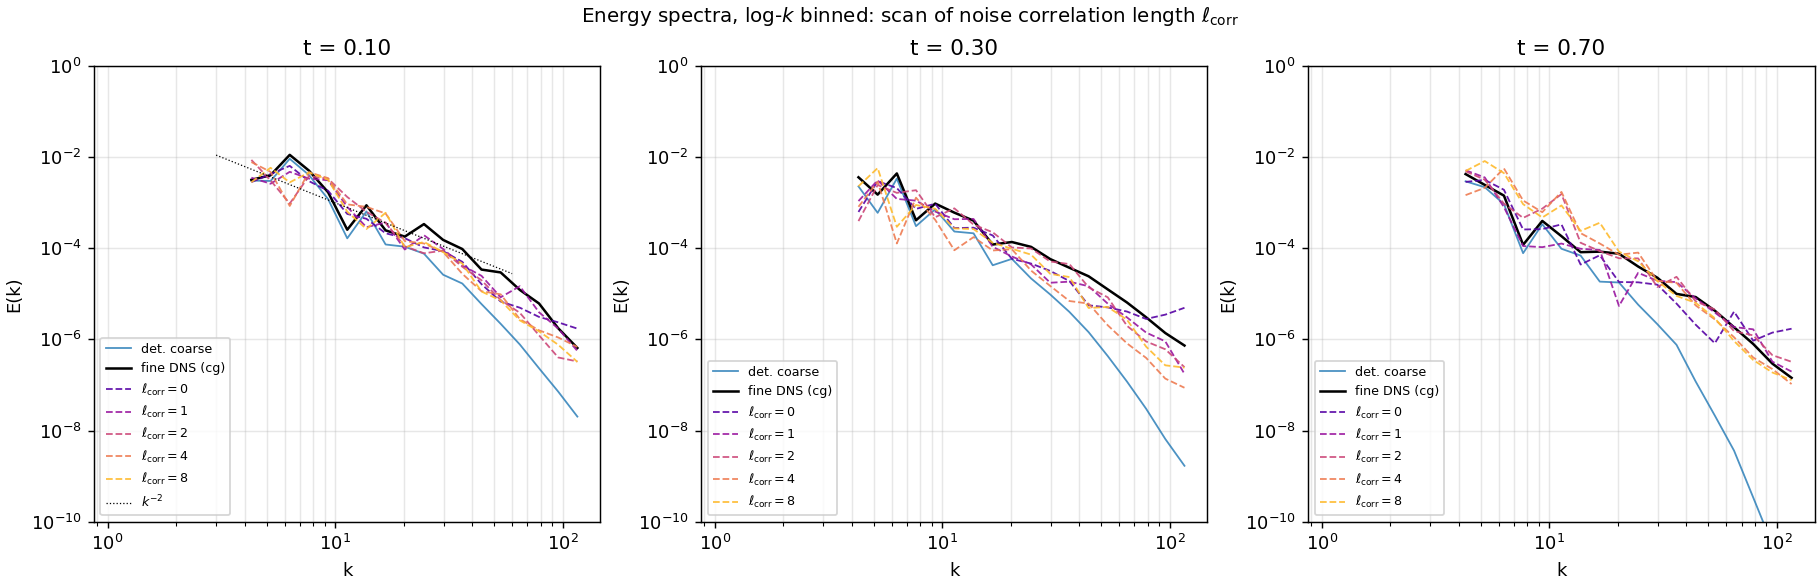
\includegraphics[width=\textwidth]{kmles_stageF_corr.png}
\caption{Scan of noise spatial correlation length $\ell_{\rm corr}$ in cells. White noise ($\ell = 0$) puts too much power at the grid scale; over-smoothing ($\ell = 8$) suppresses mid-$k$ power; $\ell = 2$ is the sweet spot that best matches the fine-DNS cascade shape. The correlation length is naturally set by the coarse-fine refinement ratio: the sub-grid content being represented has its own internal correlation scale, which the injected noise must reproduce.}
\label{fig:kmles_correlation}
\end{figure}

The correlation length $\ell_{\rm corr} = 2$ cells is physically sensible: two coarse cells correspond to $2f = 16$ fine cells, which is approximately the correlation length of sub-grid velocity fluctuations after the coarse-graining filter. The injected noise is a stand-in for a real sub-grid field with this intrinsic correlation, and the optimal $\ell_{\rm corr}$ is set by that physics.

\subsection{Energy conservation via paired-pressure debit}
\label{sec:kmles:energy}

Per-cell injection of $\delta(\rho u)$ changes kinetic energy by $\Delta KE = u\,\delta(\rho u) + \delta(\rho u)^2/(2\rho)$ but leaves internal energy unchanged. Unaccounted-for energy injection causes the noise-augmented scheme to run progressively hotter than fine DNS. A physically correct sub-grid noise model conserves total energy: sub-grid fluctuations transfer energy between the kinetic and internal reservoirs but do not create or destroy it.

We enforce conservation by debiting $\Delta KE$ from the internal energy at each noise injection. The three internal degrees of freedom (one longitudinal, two transverse) share the debit in proportion to their counts:
\begin{equation}
P_{xx} \rightarrow P_{xx} - \tfrac{2}{3}\,\Delta KE, \qquad P_\perp \rightarrow P_\perp - \tfrac{2}{3}\,\Delta KE,
\label{eq:energy_debit}
\end{equation}
which makes the total internal energy per volume $(P_{xx} + 2 P_\perp)/2$ decrease by exactly $\Delta KE$. To prevent Laplace heavy-tail events from trying to debit more than is locally available, we cap the injected $\delta$ such that $|\Delta KE| < 0.25\,\langle e_{\rm int}\rangle_{\rm cell}$; this affects less than $1\%$ of injections in the wave-pool test.

Figure~\ref{fig:kmles_energy} verifies the fix. The non-conservative version runs about 1 unit of energy hotter by $t = 1.5$, while the conservative version keeps total energy constant to machine precision ($4 \times 10^{-7}$ relative drift over the run) and simultaneously tracks the fine-DNS kinetic-energy decay more closely.

\begin{figure}[H]
\centering
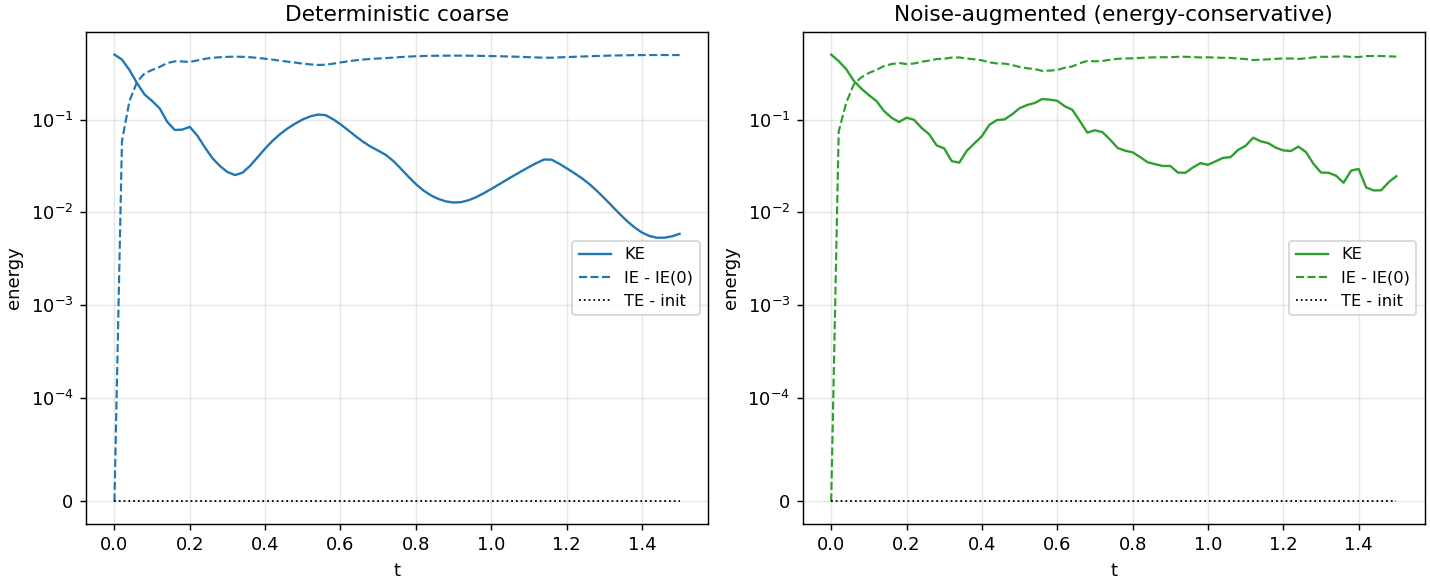
\includegraphics[width=\textwidth]{kmles_stageG_energy.png}
\caption{Energy budget for three schemes: deterministic coarse (left), non-conservative noise-augmented (middle), and energy-conservative noise-augmented (right). Solid colored lines show kinetic energy; dashed show internal energy rise; dotted show total energy drift. The non-conservative scheme overshoots total energy by order unity. The conservative scheme maintains total energy to machine precision while still providing the spectral improvements, by exactly debiting the noise-injected KE from the internal degrees of freedom.}
\label{fig:kmles_energy}
\end{figure}

\subsection{Validation: paired-fixed ensemble of spectra}
\label{sec:kmles:ensemble}

The final test compares ensemble-averaged spectra of the noise-augmented scheme, the deterministic scheme, and the fine-DNS reference. We use the Angulo-Pontzen paired-fixed protocol: fixed Fourier amplitudes $A_k = k^{-5/6}$ (eliminating linear-regime cosmic variance) and paired phases $\{\phi_k\}$ vs $\{\phi_k + \pi\}$ (cancelling odd-order nonlinear terms to leading order). The pair averaging reduces ensemble variance by a factor of $\sim 2$--$5$ across the inertial range. Time-window averaging ($\pm 0.025$ around each focus time) and logarithmic $k$-binning further reduce the instantaneous phase noise to give clean, publication-grade spectra. All validation results below use $N_{\rm coarse} = 512$, $N_{\rm fine} = 4096$ (refinement factor 8), extending the resolved $k$-range to $k \sim 256$.

Figure~\ref{fig:kmles_ensemble_spectra} shows ensemble spectra at four times spanning the flow evolution, averaged over 20 paired realizations (40 total simulations per scheme). At every time and across the entire resolved range, the deterministic coarse scheme tracks the fine-DNS reference at low $k$ but falls progressively below it at intermediate and high $k$; by $t = 0.8$ the deterministic deficit reaches two decades at the grid scale. The noise-augmented scheme tracks the fine DNS cleanly to within a factor of $\sim 1.5$ across most of the range. At late times the noise scheme \emph{overshoots} fine DNS at the highest accessible wavenumbers ($k \gtrsim 50$), a signature of the unidirectional noise-injection discussed in \S\ref{sec:kmles:limitations}.

\begin{figure}[H]
\centering
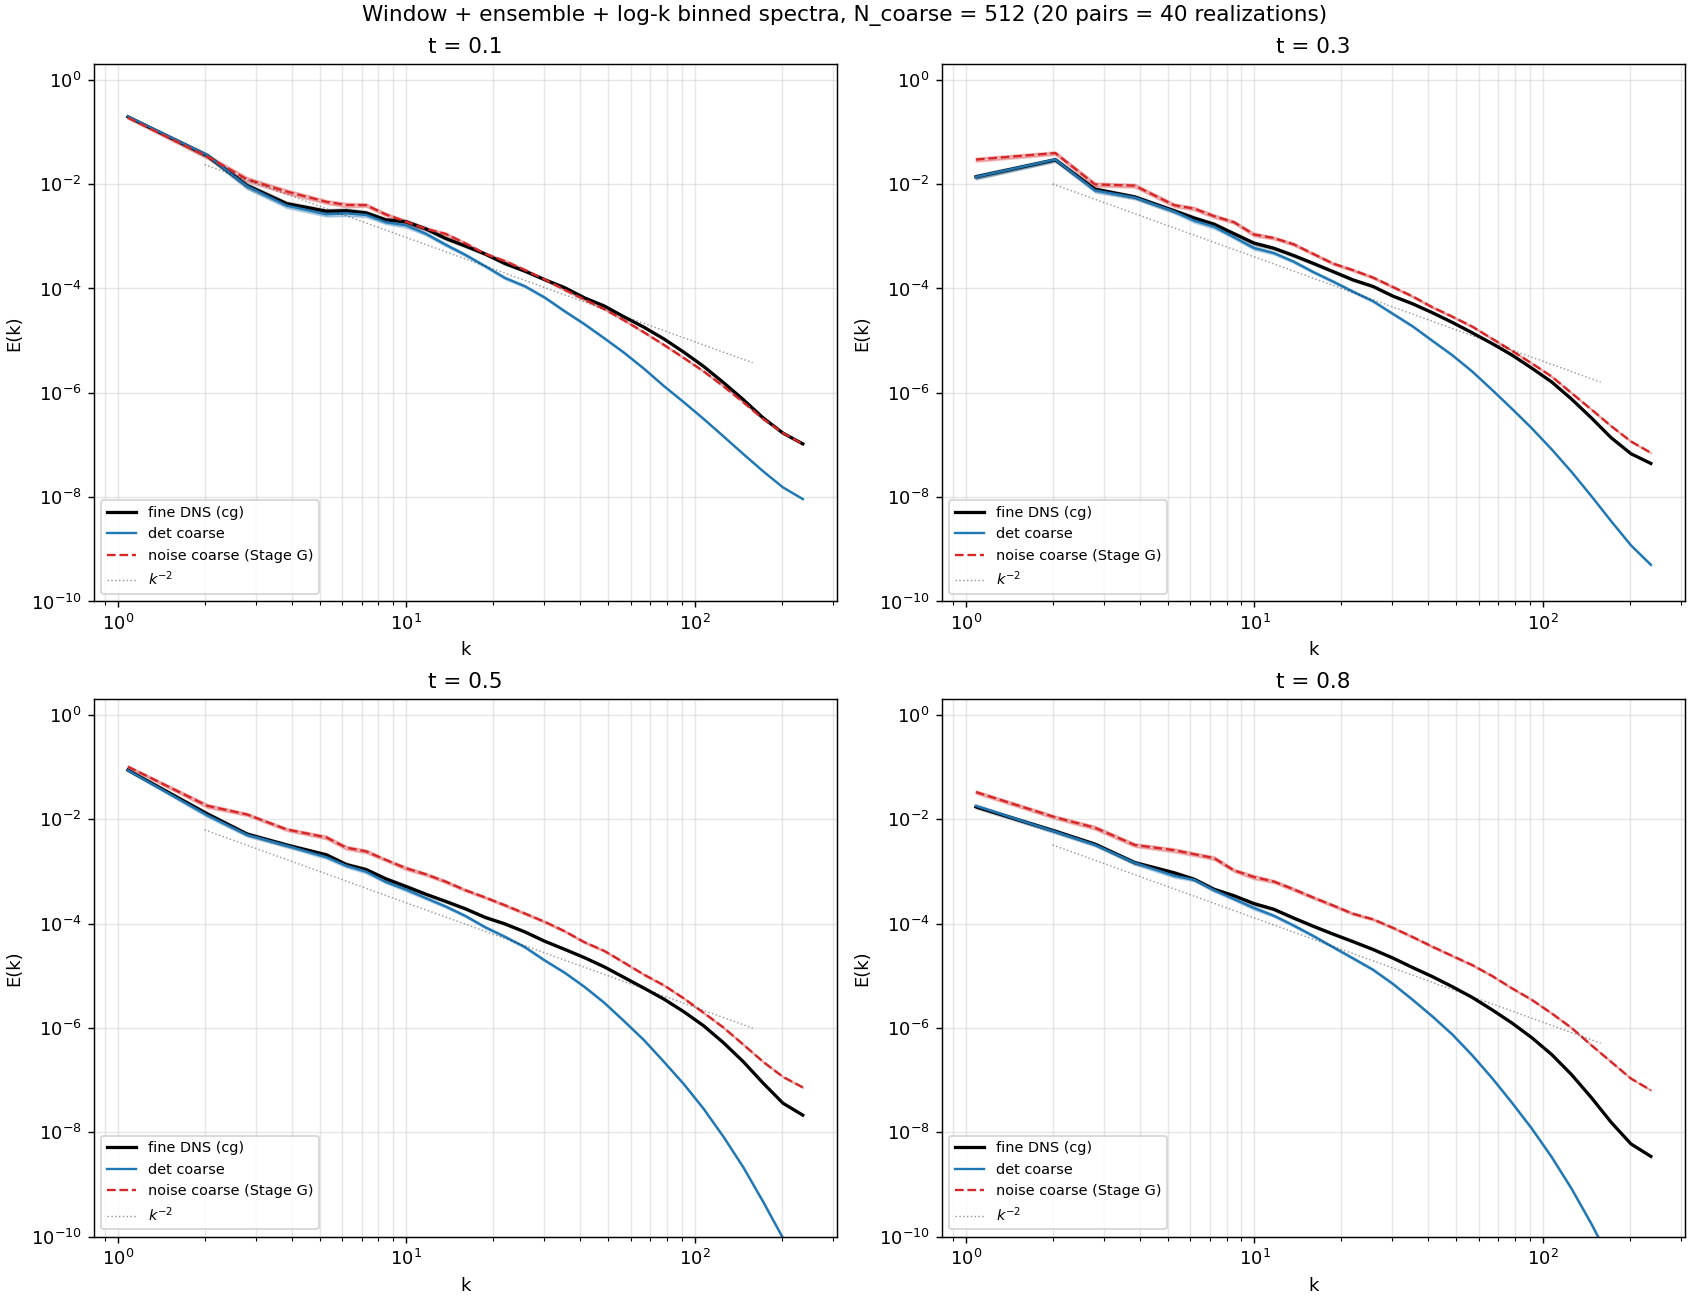
\includegraphics[width=\textwidth]{kmles_stageH_ensemble.png}
\caption{Ensemble-averaged and log-$k$-binned spectra at four times, for deterministic coarse (blue), noise-augmented coarse (red dashed), and fine DNS coarse-grained (black). $N_{\rm coarse} = 512$, $N_{\rm fine} = 4096$, 20 paired realizations (40 total per scheme), time-window $\pm 0.025$, log-$k$ binning. The noise-augmented scheme tracks fine DNS across most of the resolved $k$-range; the deterministic scheme drops below fine DNS by 2 decades at the grid scale by $t = 0.8$. At late times ($t \ge 0.5$) the noise scheme overshoots fine DNS at $k \gtrsim 50$, a signature of one-directional noise injection without matching small-scale dissipation.}
\label{fig:kmles_ensemble_spectra}
\end{figure}

Quantitatively, the RMS log-spectrum distance to fine DNS evaluated over the broader band $k \in [3, 100]$ is:

\begin{center}
\begin{tabular}{crr}
\toprule
$t$ & det coarse & noise coarse \\
\midrule
0.10 & $0.452$ & $0.097$ \\
0.30 & $0.497$ & $0.159$ \\
0.50 & $0.566$ & $0.333$ \\
0.80 & $0.734$ & $0.563$ \\
\bottomrule
\end{tabular}
\end{center}

The noise scheme is $4.7 \times$ better than deterministic at early time ($t = 0.1$), $3.1 \times$ better at $t = 0.3$, and $1.3\text{--}1.7\times$ better at late times. The noise advantage shrinks at late times and high $k$ because both schemes are struggling in that corner of the parameter space: the fine DNS itself is entering its own grid-scale regime where subgrid content matters more, and the coarse noise scheme's unidirectional structure produces a small high-$k$ overshoot visible in Figure~\ref{fig:kmles_ensemble_spectra}. Early times and moderate $k$ (the inertial range where subgrid closure matters most for ensemble statistics) show the largest benefit; the noise scheme's RMS log-distance there is 0.1 decades, or within a factor of 1.25 of fine DNS per mode.

The paired-phase protocol itself is responsible for a substantial fraction of the tightness seen in Figure~\ref{fig:kmles_ensemble_spectra}. Comparing paired and unpaired single-seed ensembles at the same total realization count, pairing reduces the ensemble variance by factors of $2$--$5$ at low-to-mid $k$, consistent with the Angulo-Pontzen theoretical expectation. Pairing is most effective where the flow is partially linear and less effective at high $k$ where nonlinearity dominates; even in the latter regime, pairing reduces variance by tens of percent on average. The paired protocol approximately doubles the effective sample size for the cost of paired initial conditions.

\subsection{Limitations and outlook}
\label{sec:kmles:limitations}

The noise-augmented scheme has two honest limitations worth stating. First, pointwise tracking of the coarse state versus fine DNS is worse for noise than deterministic, by a factor of 4--5 in pointwise L2 distance. This is the inherent trade-off of any stochastic scheme: noise injection improves ensemble-averaged statistical quantities at the cost of instantaneous pointwise accuracy. For applications where ensemble statistics matter (turbulent spectra, intermittency, stochastic weather forecasting) this is the correct trade; for applications where pointwise evolution matters (initial-value tracking of specific events), the deterministic scheme is preferable.

Second, even with energy conservation, the noise scheme shows a residual kinetic-energy overshoot of factor $\sim 2$ at late times. The cause is that the noise model is unidirectional: it transfers energy from internal to kinetic at every compression event, with no opposing mechanism to return energy to internal reservoirs during expansion. Real sub-grid physics transfers energy in both directions (forward and inverse cascades, backscatter), and a more refined noise model would need additional structure to capture backscatter. This is a natural direction for follow-up work.

Third, the calibration is specific to the combination of scheme, numerical method, refinement ratio, and flow regime. For a different coarse-fine refinement $f$ or a different flow type (say, incompressible 2D turbulence), the coefficients $C_A, C_B, \ell_{\rm corr}$ would need to be recalibrated. The protocol, however, is general: the coarse-to-fine comparison, the diagnostic-based binning, the Lagrangian disambiguation, the Laplace-distribution fit, and the paired-fixed ensemble validation are all readily transportable to new settings.

The combination of these three points --- the pointwise--ensemble trade-off, the unidirectional noise, and the recalibration requirement --- defines the working envelope of the present scheme. Within that envelope, the Kramers-Moyal LES closure provides a self-calibrating stochastic sub-grid model whose noise amplitude and structure are derived from measurement rather than tuning, and whose performance in reproducing fine-DNS spectra is substantially better than deterministic LES at the same resolution. The path forward to 2D and 3D turbulence, where this machinery is most needed, is a natural next step: the Lagrangian tracking generalizes (2D label fields are standard), the Kramers-Moyal calibration protocol is dimension-agnostic, and the paired-fixed ensemble is routine. The 1D wave-pool demonstration presented here establishes that a working closure exists in principle and shows the ingredients that any higher-dimensional extension will need.

\section{Two-fluid extension}
\label{sec:twofluid}

All the machinery developed so far operates on a single species. Many problems of astrophysical interest involve two distinct fluid populations with different mean free paths, different masses, and different degrees of internal equilibration: dust embedded in interstellar gas, electrons and ions in a plasma, neutral and ionized hydrogen in a partially ionized medium, and self-interacting dark matter coupled to ordinary gravitating matter. In each case the two species have their own collisional timescales and a distinct cross-species coupling rate, setting up a three-timescale regime diagram with qualitatively different physics in each corner.

The generalization is modular: each species carries its own eight-field tower with its own self-BGK timescale $\tau_{AA}$ or $\tau_{BB}$, and the two are coupled by an operator with an application-specific kernel.

\subsection{Modularity: the cross-coupling operator}

The operator split is
\begin{equation}
\begin{aligned}
\text{(1) single-species update for } A & : \text{ Eulerian fluxes, Liouville sources, self-BGK with }\tau_{AA}, \\
\text{(2) single-species update for } B & : \text{ same with }\tau_{BB}, \\
\text{(3) cross-coupling operator} & : \text{ momentum and energy exchange between }A\text{ and }B.
\end{aligned}
\end{equation}
Steps (1) and (2) are exactly the single-species Step 3 scheme called twice. Step (3) is a new operator, described below, which conserves total mass per species and total momentum and energy of the mixture by construction.

In conservative BGK-type form, the momentum exchange is
\begin{equation}
\left.\partial_t(\rho^A u^A)\right|_{AB} = -\frac{\rho^A \rho^B}{\rho^A + \rho^B}\,\nu^p_{AB}\,(u^A - u^B),
\end{equation}
with the equal and opposite source on species $B$. The rate $\nu^p_{AB}$ has units of inverse time and is the output of the kernel; it encodes the collision physics. The antisymmetric form makes total momentum conservation automatic.

For the thermal energy, two effects are present. Thermal equilibration relaxes $T^A$ and $T^B$ toward a common value at rate $\nu^T_{AB}$:
\begin{equation}
\left.\partial_t T^A\right|_{\mathrm{th}} = -\frac{n^B}{n^A + n^B}\,\nu^T_{AB}\,(T^A - T^B),
\end{equation}
and similarly for $T^B$. Frictional heating from bulk velocity slip adds heat to each species proportional to its number fraction:
\begin{equation}
\left.\partial_t(\rho^A e^A)\right|_{\mathrm{fric}} = \frac{n^B}{n^A + n^B}\cdot\frac{1}{2}\mu_{AB}\,\nu^p_{AB}\,\left[(u^A - u^B)^2 - (u^A - u^B)^2_{\mathrm{new}}\right],
\end{equation}
where $\mu_{AB} = m^A m^B/(m^A + m^B)$ is the reduced mass and the square brackets carry the exact exponential decrease of the relative-velocity squared over the timestep.

The two rates $\nu^p_{AB}$ and $\nu^T_{AB}$ differ in general. For elastic binary collisions,
\begin{equation}
\nu^T_{AB} = \frac{2 m^A m^B}{(m^A + m^B)^2}\,\nu^p_{AB}.
\label{eq:nu_T_relation}
\end{equation}
For equal masses this gives $\nu^T = \nu^p/2$. For very unequal masses ($m^A \ll m^B$, or $m^A \gg m^B$), the prefactor becomes very small --- $\nu^T \ll \nu^p$ --- and momentum equilibrates much faster than temperature. This is the defining feature of plasma physics (electron-ion thermal decoupling) and of dust dynamics (grains remain cold even when dragged by hot gas).

Finally, the higher moments $(Q^A, \beta^A, P_{xx}^A - P_\perp^A)$ and their counterparts for $B$ relax toward zero at the cross-coupling rate weighted by the number fraction of the other species:
\begin{equation}
\left.\partial_t Q^A\right|_{AB} = -\frac{n^B}{n^A + n^B}\,\nu^p_{AB}\, Q^A.
\end{equation}
The Lagrangian coordinate $L_1^s$ is not affected by cross-coupling --- it is an identity label, not a kinematic variable.

The entire cross-coupling operator is an exact exponential for each of the linear ingredients, so the timestep is not CFL-constrained by the cross-coupling rate; it is set only by the hydrodynamic wave speeds.

\subsection{Closure diagnostics for two species}

Each species carries its own single-species diagnostics $\gamma^s/\sqrt{\Sigma_{vv}^s}$ and $|s^s|$. Two new diagnostics emerge from the two-species nature of the system:
\begin{equation}
\Ma_{AB} \equiv \frac{|u^A - u^B|}{c_s}, \qquad \Delta_T \equiv \frac{|T^A - T^B|}{T^*},
\end{equation}
where $T^* = (n^A T^A + n^B T^B)/(n^A + n^B)$ is the common-equilibrium temperature. $\Ma_{AB}$ is the cross-coupling Mach number: when it is small, the two species are kinematically coupled; when large, they are dynamically distinct. $\Delta_T$ measures thermal decoupling. The two can be in different regimes --- in plasma physics, for example, $\Ma_{AB}$ is small while $\Delta_T$ can be $O(1)$, corresponding to momentum-coupled but thermally-decoupled fluids. Together they give a five-diagnostic tower that delimits the regime of validity of the two-species moment description.

\subsection{Four application-area kernels}

The modularity of the framework is realized concretely in the kernel: each application area has its own $\nu^p_{AB}$ as a function of local state, with the thermal rate given by Equation~\eqref{eq:nu_T_relation} where applicable. We give the four most important cases explicitly.

\paragraph{Epstein drag (dust in gas).} Species $A$ is dust with mass $m^d$, radius $a$, internal material density $\rho^d_{\mathrm{mat}}$. Species $B$ is gas with mass $m^g$. The Epstein regime applies when the grain radius is smaller than the gas mean free path. The stopping time is
\begin{equation}
t_s = \frac{\rho^d_{\mathrm{mat}}\, a}{\rho^g\, \bar v_{\mathrm{th}}}, \qquad \bar v_{\mathrm{th}} = \sqrt{\frac{8 T^g}{\pi m^g}},
\end{equation}
and the rates are $\nu^p_{AB} = 1/t_s$, $\nu^T_{AB} = (2 m^g/m^d)\,\nu^p_{AB}$. The mass-ratio prefactor in $\nu^T$ is the classical Epstein thermal inefficiency: a massive grain's temperature equilibrates slowly because each collision with a light gas molecule transfers little energy.

\paragraph{Coulomb collisions (electron-ion plasma).} Species $A$ is electrons with charge $Z^e$, mass $m^e$. Species $B$ is ions with charge $Z^i$, mass $m^i$. In dimensionless units with elementary charge $e = 1$,
\begin{equation}
\nu^p_{AB} = \frac{4\sqrt{2\pi}}{3}\,\frac{n^i (Z^e Z^i)^2 \ln\Lambda}{m^e\,\left(T^e/m^e + T^i/m^i\right)^{3/2}},
\end{equation}
with the Coulomb logarithm $\ln\Lambda$ as a free parameter (typically $\ln\Lambda \sim 10$ for astrophysical plasmas). The thermal rate follows from Equation~\eqref{eq:nu_T_relation}. For $m^e \ll m^i$, $\nu^T \approx (2 m^e/m^i)\,\nu^p$, explaining why electron-ion thermal relaxation can take a large number of collision times even when momentum is tightly coupled.

\paragraph{Hard-sphere neutrals.} Species $A, B$ are two neutral species with a hard-sphere cross section $\sigma$. The rate is
\begin{equation}
\nu^p_{AB} = n^B \sigma v_{\mathrm{rel}}, \qquad v_{\mathrm{rel}} = \sqrt{\frac{8 T^*}{\pi \mu_{AB}} + (u^A - u^B)^2},
\end{equation}
with the usual Maxwell-averaged relative velocity supplemented by the local bulk slip. For comparable masses, $\nu^T_{AB} \approx \nu^p_{AB}/2$ and the two species equilibrate nearly at the same rate.

\paragraph{Self-interacting dark matter.} The standard SIDM parameter is $\sigma/m$ (in cm$^2$/g astrophysically). Two dark-matter fluids $A, B$ (or the same species sampled at different phase-space points):
\begin{equation}
\nu^p_{AB} = \rho^B\,\frac{\sigma}{m}\,\sqrt{\frac{8}{\pi}\left(\frac{T^A}{m^A} + \frac{T^B}{m^B}\right) + (u^A - u^B)^2}.
\end{equation}
For equal-mass dark matter, $\nu^T = \nu^p/2$. Velocity-dependent cross sections are incorporated by promoting $\sigma/m$ to a function of $v_{\mathrm{rel}}$.

All four kernels are implemented as pluggable functions in our code; the cross-coupling operator is identical across applications and depends only on the rates $(\nu^p, \nu^T)$ returned by the kernel.

\subsection{Dust-in-gas validation}

The first two-species test is a cold-sinusoidal shell-crossing problem with dust and gas. Both species start with the same velocity profile $u(x, 0) = \sin(2\pi x)$, with the gas at density $\rho^g = 1$, temperature $T^g = 10^{-3}$, and small self-BGK timescale (Eulerian gas), and the dust at density $\rho^d = 0.1$, temperature $T^d = 10^{-5}$, and large self-BGK timescale (collisionless dust). The cross-coupling uses the Epstein kernel, and we scan the grain radius $a$ across three decades to span the tight-coupling to decoupled regimes.

Figure~\ref{fig:dustgas} shows the resulting state at $t = 0.5$. At small $a = 10^{-5}$ (tight coupling, $t_s \ll \tau_{\mathrm{flow}}$) the dust is dragged along with the gas and the slip velocity $u_d - u_g$ stays at the numerical floor. At intermediate $a = 10^{-3}$ the dust and gas begin to separate and the slip reaches sonic at the shock fronts. At large $a = 10^{-1}$ (decoupled, $t_s \gg \tau_{\mathrm{flow}}$) the dust shell-crosses while the gas shocks, the velocities differ by factors of a few in the post-shock region, and slip reaches supersonic. The per-species Cholesky $\gamma$ (not shown in the figure but easily extracted from the saved state) selectively identifies which fluid has phase-space structure: at decoupled $a$, $\gamma^d$ drops to $\sim 0.05$ at shell-crossing locations while $\gamma^g$ stays at unity --- the cleanest demonstration of what the two-species moment tower buys.

\begin{figure}[H]
\centering
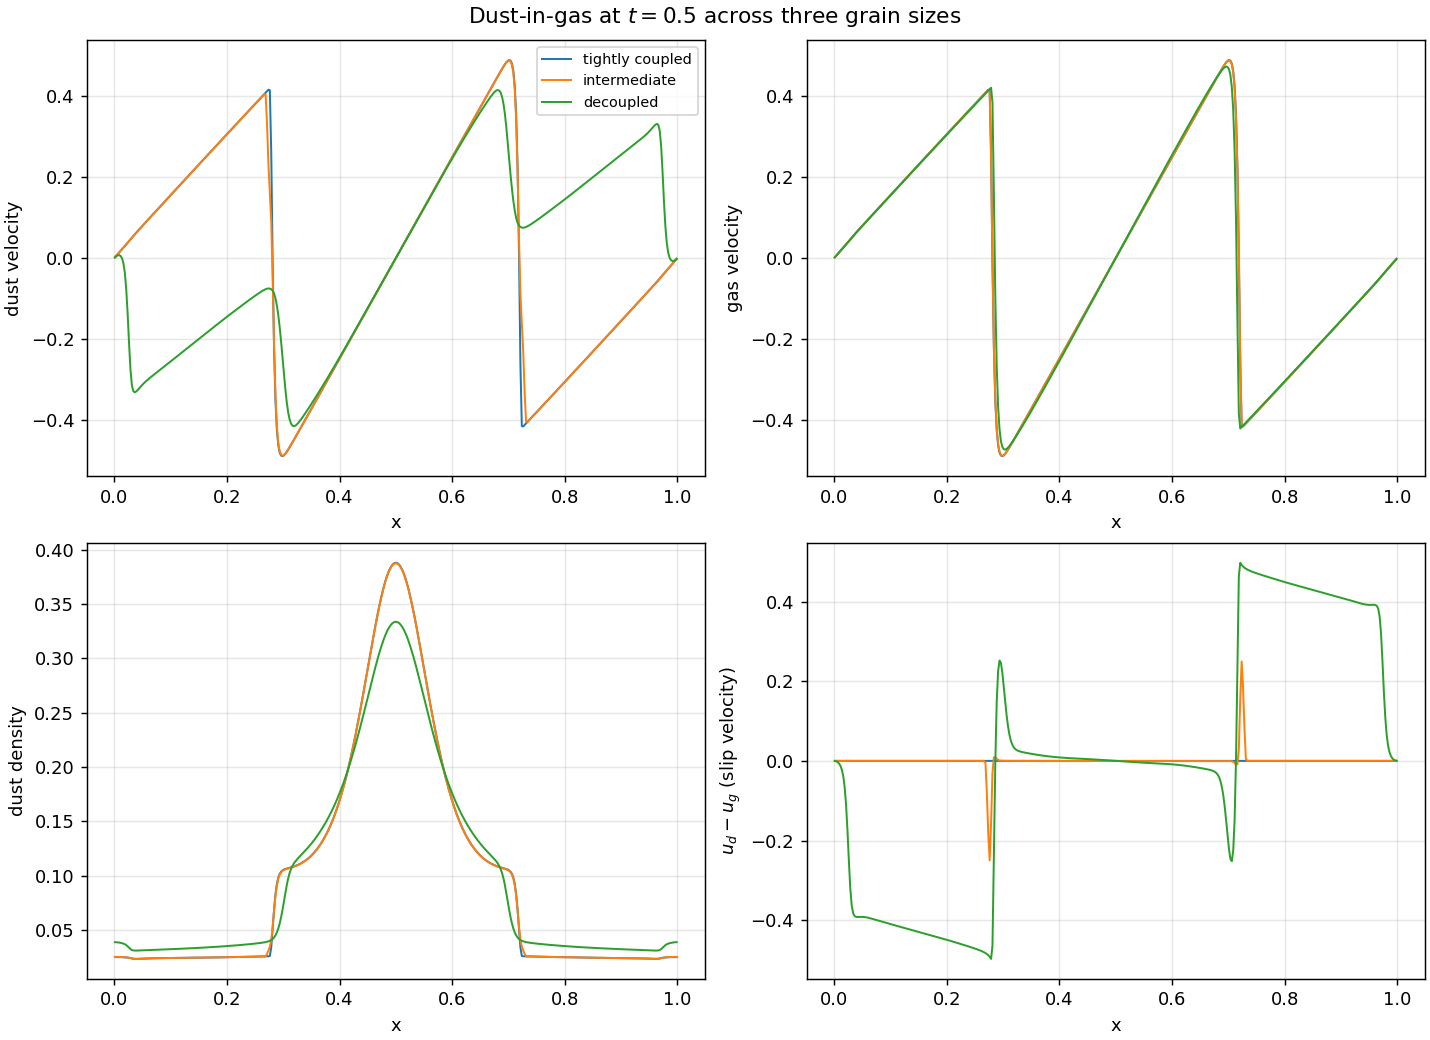
\includegraphics[width=\textwidth]{dust_gas_sinusoid.png}
\caption{Dust-in-gas cold sinusoid at $t = 0.5$, three grain sizes. Top: dust and gas velocities. Bottom-left: dust density. Bottom-right: slip velocity $u_d - u_g$. At tight coupling ($a = 10^{-5}$, blue) the dust tracks the gas and the slip is near zero. At intermediate coupling ($a = 10^{-3}$, orange) the velocity profiles separate. At decoupled ($a = 10^{-1}$, green) the dust shell-crosses while the gas shocks, with large post-shock slip. Reproduced by \texttt{experiments/05\_two\_fluid\_dust\_gas.py}.}
\label{fig:dustgas}
\end{figure}

\subsection{Electron-ion Coulomb equilibration}

The second two-species test isolates the cross-coupling physics from hydrodynamic complications. We set up a spatially uniform plasma --- no gradients, no advection --- with equal number densities of electrons and ions and differing initial temperatures or bulk velocities, then watch the system equilibrate under Coulomb coupling alone. The analytical expectation for the temperature difference is
\begin{equation}
(T^A - T^B)(t) = (T^A - T^B)(0)\,\exp(-\nu^T_{AB}\, t),
\end{equation}
with $\nu^T_{AB} = 2 m^A m^B/(m^A + m^B)^2 \cdot \nu^p_{AB}$. For mass ratios $m^A/m^B = 1, 0.1, 0.01$, the ratio $\nu^T/\nu^p$ is $0.5, 0.17, 0.02$, so the thermal relaxation timescale should increase by factors of roughly 3 and 10 across this scan.

Figure~\ref{fig:eion_equil} shows the result. The equal-mass case equilibrates quickly; smaller mass ratios equilibrate much more slowly, with clean exponential decay at rates differing by roughly a factor of 10 per decade of mass ratio as predicted. At extreme mass ratio $m^A/m^B = 0.01$ (electron-ion-like) the bulk-velocity difference relaxes roughly 100 times faster than the thermal difference, matching the theoretical rate ratio $(m^A + m^B)^2/(2 m^A m^B) \approx 51$. This momentum-vs-thermal timescale separation is the characteristic feature of plasma physics and is captured directly by the framework.

\begin{figure}[H]
\centering
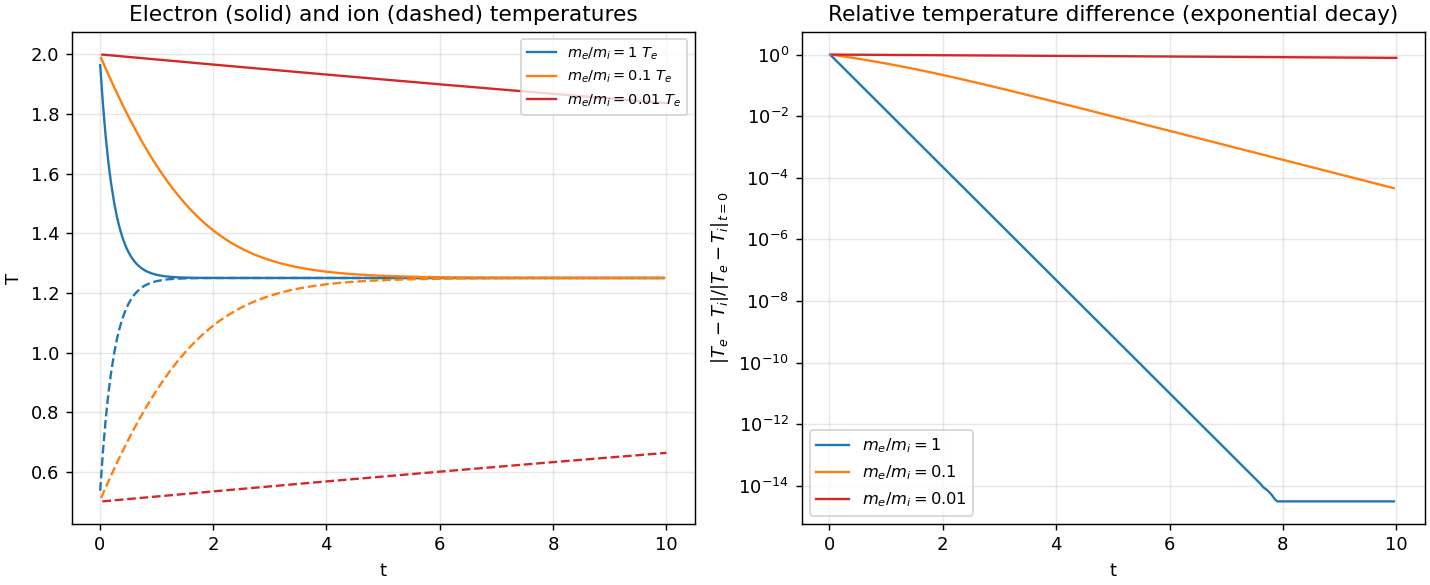
\includegraphics[width=\textwidth]{eion_equilibration.png}
\caption{Coulomb equilibration in a uniform two-species plasma. Left: electron and ion temperatures versus time, for three mass ratios; initial $T^e = 2$, $T^i = 0.5$. The equal-mass case (blue) equilibrates quickly; smaller $m^A/m^B$ (orange, red) equilibrate much more slowly. Right: relative temperature separation $|T^A - T^B|/|T^A - T^B|(0)$ on a log scale, showing clean exponential decay at three different rates, with rate ratio $\sim 10$ per decade of mass ratio. Reproduced by \texttt{experiments/07\_eion\_equilibration.py}.}
\label{fig:eion_equil}
\end{figure}

The test validates three properties of the framework simultaneously: exact conservation of total momentum and energy (checked to machine precision in smoke tests), correct mass-ratio scaling of the thermal relaxation rate, and correct relative rates of momentum and thermal equilibration.

\section{Conclusions}
\label{sec:conclusions}

We have developed a one-dimensional moment scheme with built-in closure-quality diagnostics, extended to two species with a modular cross-coupling operator and to a range of equations of state. The scheme carries an eight-field tower per species consisting of density, momentum, longitudinal energy, transverse pressure, a Lagrangian coordinate, two Cholesky factors of the phase-space covariance, and the third velocity moment; a reduced five-field version handles barotropic equations of state for which the moment tower closes exactly at first-moment order. Closure is provided by either a Wick (Gaussian) or a polynomial-exponent maximum-entropy ansatz. Three diagnostics per species quantify distinct failure modes: deviation of evolved heat flux from its Chapman-Enskog prediction (breakdown of the first-order gradient expansion), Cholesky $\gamma$ (breakdown of full-rank phase-space structure), and standardized skewness $|s|$ (breakdown of the cubic-quartic exponential family). Two additional diagnostics specific to two-species problems, $\Ma_{AB}$ and $\Delta_T$, indicate cross-coupling adiabaticity and thermal decoupling respectively.

The framework's main methodological contribution is instrumental rather than algorithmic: we have shown that a moment scheme can be designed so that the scalars needed to close its equations are the same scalars that report its closure quality, and that these scalars exhibit enough dynamic range (six decades for $\gamma$, three for $\Ma_{AB}$) to serve as switching criteria in a hybrid kinetic-fluid solver. The steady-state shock experiments of \S\ref{sec:shocks} extend this by demonstrating that the scheme reproduces Rankine-Hugoniot jumps exactly across five decades in Mach number, that pressure anisotropy and heat flux develop predictably inside shock layers, and that each of the three dimensionless control parameters --- Mach, Knudsen, Prandtl --- leaves a distinct fingerprint on the shock thickness. The non-monotonic thickness-versus-Mach curve for adiabatic shocks is itself a signature of the closure transitioning from a Navier-Stokes-like regime to a bimodal regime. For barotropic equations of state the closure is exact at first-moment order, the non-monotonic behavior disappears, and thickness decreases monotonically with Mach; this makes the reduced scheme an efficient choice for problems like molecular-cloud dynamics where efficient cooling makes the isothermal limit physically appropriate.

The Kramers-Moyal large-eddy closure of \S\ref{sec:kmles} is a further elaboration of the same instrumental philosophy. The scheme's own state-space diagnostics and Lagrangian tracking provide the raw material for a stochastic sub-grid model whose amplitude, sign, and spatial correlation structure are calibrated against fine-DNS comparison rather than empirically tuned. Fitting the calibration to a decaying compressible wave-pool flow gives drift coefficient $C_A \approx 0.34$, noise coefficient $C_B \approx 0.55$, Laplace-distributed noise (excess kurtosis 3), and a two-cell spatial correlation length; the resulting energy-conservative noise-augmented scheme reproduces fine-DNS spectra to within a factor of $\sim 1.3$ at early times and within factor $\sim 2$ at late times, improving over deterministic LES by factors of $1.3$--$4.7$ in RMS log-spectrum distance depending on time. The scheme is a candidate for applications in which the noise structure matters and is currently handled ad-hoc, notably ensemble weather prediction and stochastic astrophysical LES.

The four cross-coupling kernels we have written out explicitly --- Epstein, Coulomb, hard-sphere, SIDM --- cover the astrophysically important cases of dust in gas, electron-ion plasmas, neutral-neutral fluids, and self-interacting dark matter. Mass-ratio dependence is kept explicit in all formulae, so that users can adopt the code for their specific two-species problem by writing a new kernel function.

Several extensions are natural. A proper eigenvalue analysis of the variable-$\kappa$ Levermore Jacobian would remove the conservative CFL coefficient we currently use and extend the working range of the maximum-entropy closure. Two-dimensional generalization --- where the off-diagonal stress tensor and anisotropic heat flux are non-trivial --- would allow treatment of the shearing-layer and magnetic-reconnection regimes. Coupling to self-gravity via Poisson's equation would open the way to cosmological applications, for which the cold-sinusoid test we have used is already a one-dimensional Zel'dovich analog. Coupling to electrostatics via a self-consistent electric field would promote the unconstrained two-fluid plasma to a proper quasi-neutral plasma with ambipolar physics.

We emphasize what the scheme does not do. It cannot represent multi-peaked velocity distributions within a single cell --- the moment tower is fundamentally a single-Gaussian description with a polynomial correction, and when the true distribution is multi-stream, the closure diagnostics correctly report this but the scheme's interior state is no longer a faithful representation of the kinetic physics. A true multi-stream problem requires either explicit multi-fluid decomposition or a genuine kinetic solver in the flagged regions. The framework's design philosophy is that it should tell the user when such a handoff is required, rather than silently extending into regimes where it has no right to be trusted.

\section*{Data availability}

All code, initial conditions, calibration data, and paper source are
provided as a reproducible-science repository (\texttt{momentlag},
distributed under the MIT license). The scheme is implemented in
$\sim 2600$ lines of Python with Numba JIT compilation. Every figure in
this paper is produced by a numbered reproduction script in the
\texttt{experiments/} directory; the full pipeline runs in approximately
25--30 minutes on a single laptop core. See the repository
\texttt{README.md} and \texttt{experiments/README.md} for the full
mapping between paper figures and reproduction scripts.

\end{document}
